\documentclass[conference]{IEEEtran}
% \IEEEoverridecommandlockouts
% The preceding line is only needed to identify funding in the first footnote. If that is unneeded, please comment it out.
%Template version as of 6/27/2024

\usepackage{cite}
\usepackage{amsmath,amssymb,amsfonts}
\usepackage{graphicx}
\usepackage{textcomp}   
\usepackage{xcolor}
\usepackage{algorithm}
\usepackage{algpseudocode}
% \usepackage{hyperref}
\usepackage[colorlinks=true, linkcolor=blue, citecolor=blue, urlcolor=blue]{hyperref}

\def\BibTeX{{\rm B\kern-.05em{\sc i\kern-.025em b}\kern-.08em
    T\kern-.1667em\lower.7ex\hbox{E}\kern-.125emX}}

\newcommand{\nsnote}[1] {{$\langle${\textcolor{blue}{NS: \textbf{#1}}}$\rangle$}}
\begin{document}

\title{Cooperative Wind Gradient Estimation for Small UAS Formations\\
}

\author{\IEEEauthorblockN{Nolan Stevenson}
\IEEEauthorblockA{\textit{ASEN 5128: Small Unmanned Aircraft System Guidance, Navigation, and Control} \\
\textit{University of Colorado Boulder} \\
}
}

\maketitle

\begin{enumerate}
    \item \href{https://github.com/nolans12/sUAS-Final-Project}{{\textcolor{blue}{Link to GitHub Repository}}}
    \item \href{https://youtu.be/I1R92603xzI}{{\textcolor{blue}{Link to 3 UASs Estimating Wind Gradient}}}
    \item \href{https://youtu.be/PB9hqby9TCI}{{\textcolor{blue}{Link to 1 UAS, No Climb, Estimating Wind Gradient}}}
    \item \href{https://youtu.be/ZCwqw6uvsHc}{{\textcolor{blue}{Link to 1 UAS With Climb Estimating Wind Gradient}}}
\end{enumerate}

\section{Introduction and Background}

% \nsnote{alot of what happens in the Abstract}

% \nsnote{talk about how the gradient is important. how its used}

% \nsnote{talk about how suas are used to collect science data}

The goal of this paper is to investigate the feasibility of using multiple small Uncrewed Aerial Systems (UAS) to cooperatively estimate an unknown wind field. 
If multiple UAS are flying in a formation, algorithms can be implemented to allow the sensor data from each UAS to be fused together to collaboratively estimate a wind field.
The combined estimate of the wind field should be more accurate than a single UAS estimate, as formation flying allows for higher observability of the wind field; taking measurements at different temporal and spacial locations.

Accurate wind field estimation is important for many applications of UAS flight, wind energy extraction, and civil engineering. The ability to cooperatively estimate the wind field would allow small UAS to fly more efficiently, using dynamic soaring to extract energy from the wind.
Accurate wind field estimation is also critical from a science perspective; wind gradient data is critically important for the design of buildings and wind turbines arrays for maximum energy extraction \cite{abdalla2023, matiko2013, rehman2008, vasel2017}. 
Additionally, collabrative estimation allows for more robustness to failures. If one UAS or sensor malfunctions, the wind field estimation is not blocked, but just degraded. 

The current state of the art for wind field estimation is to use CFD simulations over the surface of the terrain to fit the wind gradient to the power law relationship \cite{probst2010}.
These simulations have been proven to perform well for slopes lower than $25\%$ grade. 
But, running CFD simulations is computationally expensive and time consuming. 
The agility of having a fleet of UAS to quickly survey the wind field would allow for faster wind field estimation, although it does require an in-person presence.
However, CFD simulations are way too computationally expensive to be used online in a UAS.
As mentioned above, the ability for a UAS to estimation the wind field online may allow unique explotation of the wind using dynamic and static soaring techniques.


Wind gradients vary drastically depending on weather conditions and terrain. An example of how human made buildings impact the wind gradient is shown in Figure~\ref{fig:wind_gradient_buildings}. 
This figure shows the impact terrain has on the surface roughness, $\alpha$, which is directly proportional to the wind gradient in the boundary layer.
Because of the high variablility of the wind gradient, any usage of UAS for wind field estimation must be robust and able to handle a wide range of wind gradients.

\begin{figure}[h]
    \centering
    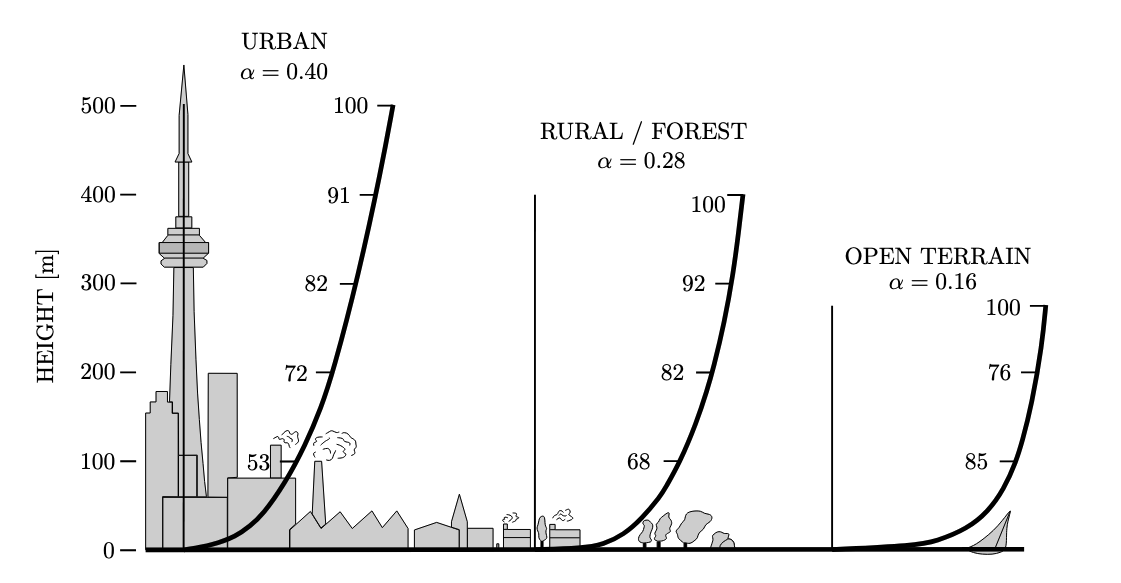
\includegraphics[width=0.5\textwidth]{images/wind_gradient_buildings.png}
    \caption{Impact of terrain on surface roughness, $\alpha$, and wind gradient, \cite{recoskie2017}}
    \label{fig:wind_gradient_buildings}
\end{figure}

This paper will explore using a robust centralized online optimizer to estimate the wind field using a series of wind measurements taken from a formation of UAS.
The pros, cons, and improvements on this approach will be discussed in detail.
\section{Problem Formulation}

\subsection{Wind Gradient Model}

As mentioned above in the background section, wind gradients can be generalized as a form of the power law, which has the following relationship:
\begin{equation}
    v_z = v_{ref} * (\frac{z}{z_{ref}})^{\alpha}  
    \label{eq:power_law}
\end{equation}

Equation~\ref{eq:power_law} follows a logarithmic relationship between the wind speed and altitude given some reference wind speed and altitude.
To abstract this into a more general form, where we dont need a reference wind speed and altitude this paper will be using the following equation for the wind gradient:
\begin{equation}
    v_{wind} (h) = a * ln(h + b)
    \label{eq:wind_gradient}
\end{equation}

Where $a$ and $b$ are constants the define the slope profile of the wind gradient. This translates to a function of $h$, the height above the ground.
Given a $h$, this returns the magnitude of the wind speed at that given height. Given a series of measurements of the wind at different heights, we can work to estimate the constants $a$ and $b$.
This allows us to estimate the wind gradient at any given height.

The large variety of wind gradients this relationship is able to capture is shown in Figure~\ref{fig:wind_gradients}.
As you can see, depending on the values of $a$ and $b$, a power law relationship can be created.

\begin{figure}[h]
    \centering
    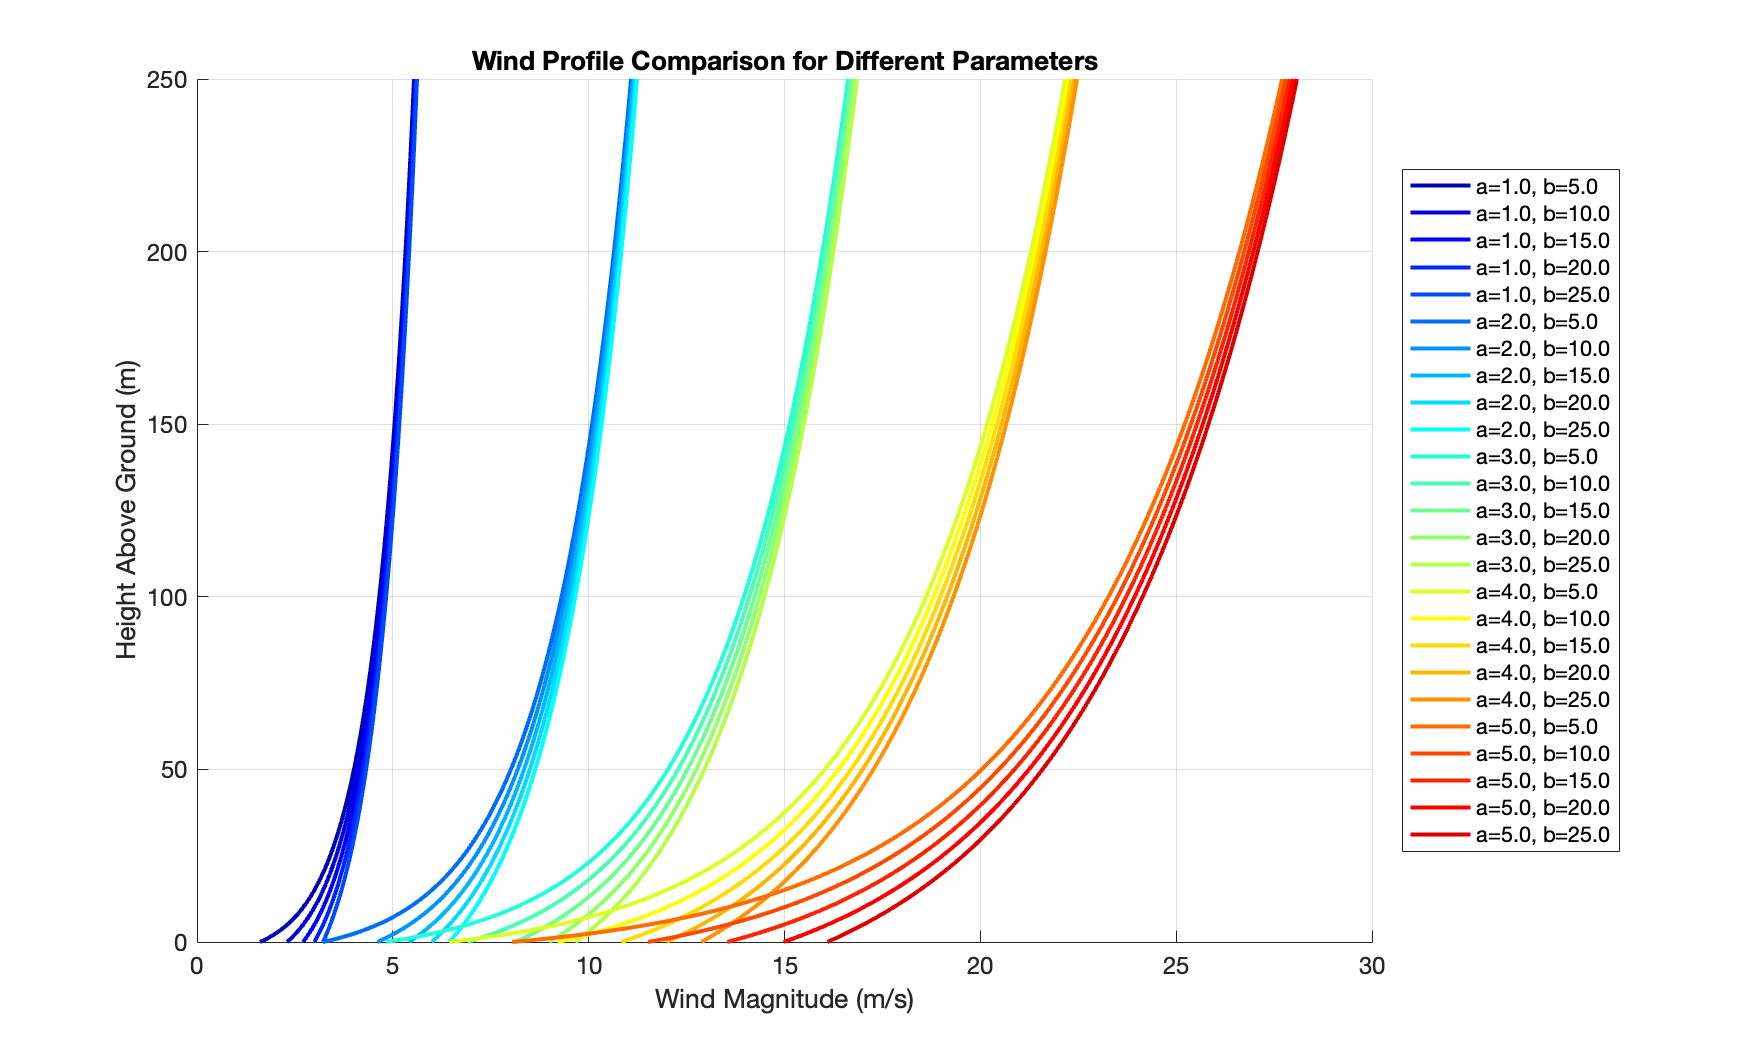
\includegraphics[width=0.6\textwidth]{images/wind_grads.png}
    \caption{Various wind gradient profiles. Comapring a and b values.}
    \label{fig:wind_gradients}
\end{figure}

\subsection{UAS Guidance Algorithm}

To measure the wind gradient, we will be using a series of UAS. These UAS will be flying a variety of straight line missions, each probing wind estimates from a different altitude. 
In order to command the UAS to follow a straight line mission, we will be using the lookahead straight line following algorithm, as given in Algorithm~\ref{alg:lookahead}.

\begin{algorithm}
    \caption{Lookahead Straight Line Following Guidance}\label{alg:lookahead}
    \begin{algorithmic}
    \State \textit{Given a current position, a line to follow (initial point and vector), and a lookhead distance, return the desired heading and velocity vector.}
    \Function{lookahead}{pos, line0, lineVec, lookahead}
    \State Calculate unit vector along line: $\hat{v} = \frac{lineVec}{||lineVec||}$
    \State Get rel pos of current to line start: $p_c = pos - line0$
    \State Project $p_c$ onto line: $p_{proj} = p_c \cdot \hat{v}$
    \State Get lookahead point: $p_{target} = line0 + (p_{proj} + lookahead) \cdot \hat{v}$
    \State Get error vector: $e = p_{target} - pos$
    \State Calculate desired heading: $\psi_d = \text{atan2}(e.y, e.x)$
    \State Calculate desired velocity vector: $v_d = \frac{e}{||e||} * ||lineVec||$
    \State Return heading and velocity vector
    \EndFunction
    \end{algorithmic}
\end{algorithm}

An image showing the visual trigonometry of the lookahead guidance algorithm for finding the target waypoint is shown in Figure~\ref{fig:lookahead}.

\begin{figure}[h]  
    \centering
    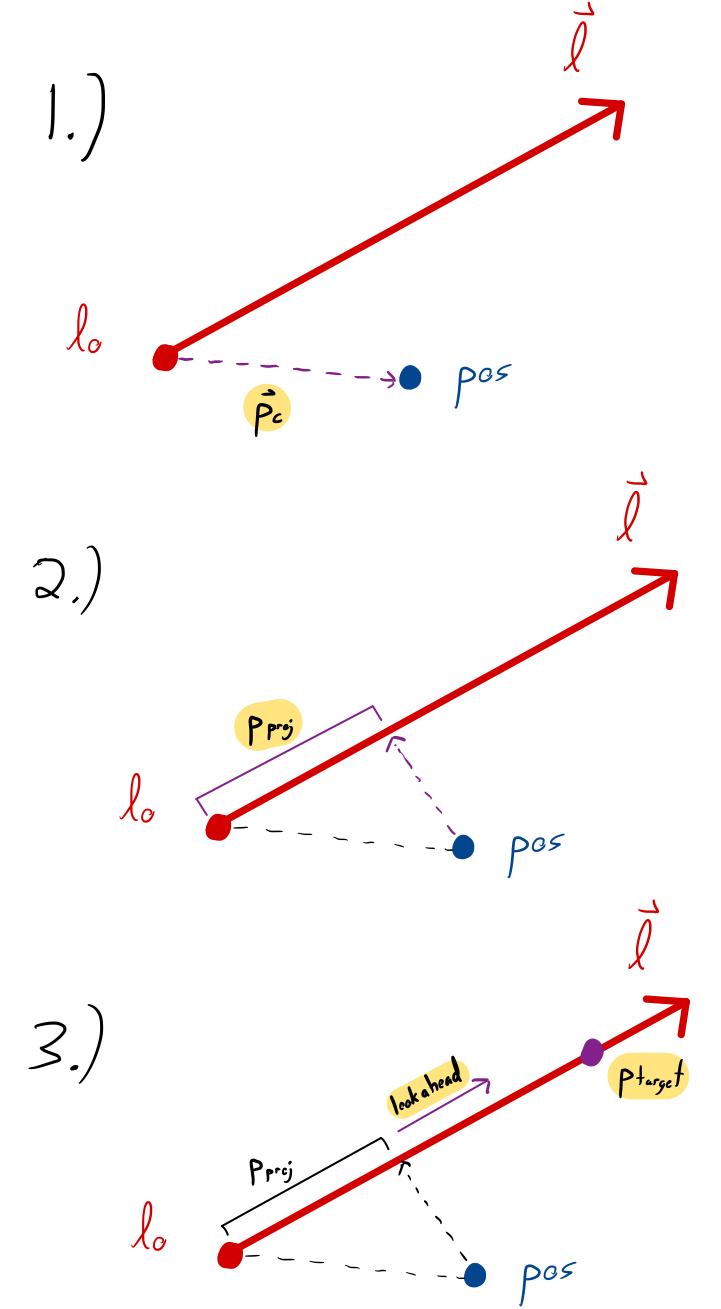
\includegraphics[width=0.35\textwidth]{images/proj_math.jpeg}
    \caption{Lookahead Guidance Trigonometry}
    \label{fig:lookahead}
\end{figure}

The autopilot a UAS uses is able to take in a desired heading, a desired height, and a desired height rate.
By taking these values from the lookahead guidance algorithm and simulating the UAS as a point mass through the vector field, through MATLAB's ode45, we get the result shown in Figure~\ref{fig:lookahead_sim} for a point mass following a guidance line:

\begin{figure}[h]  
    \centering
    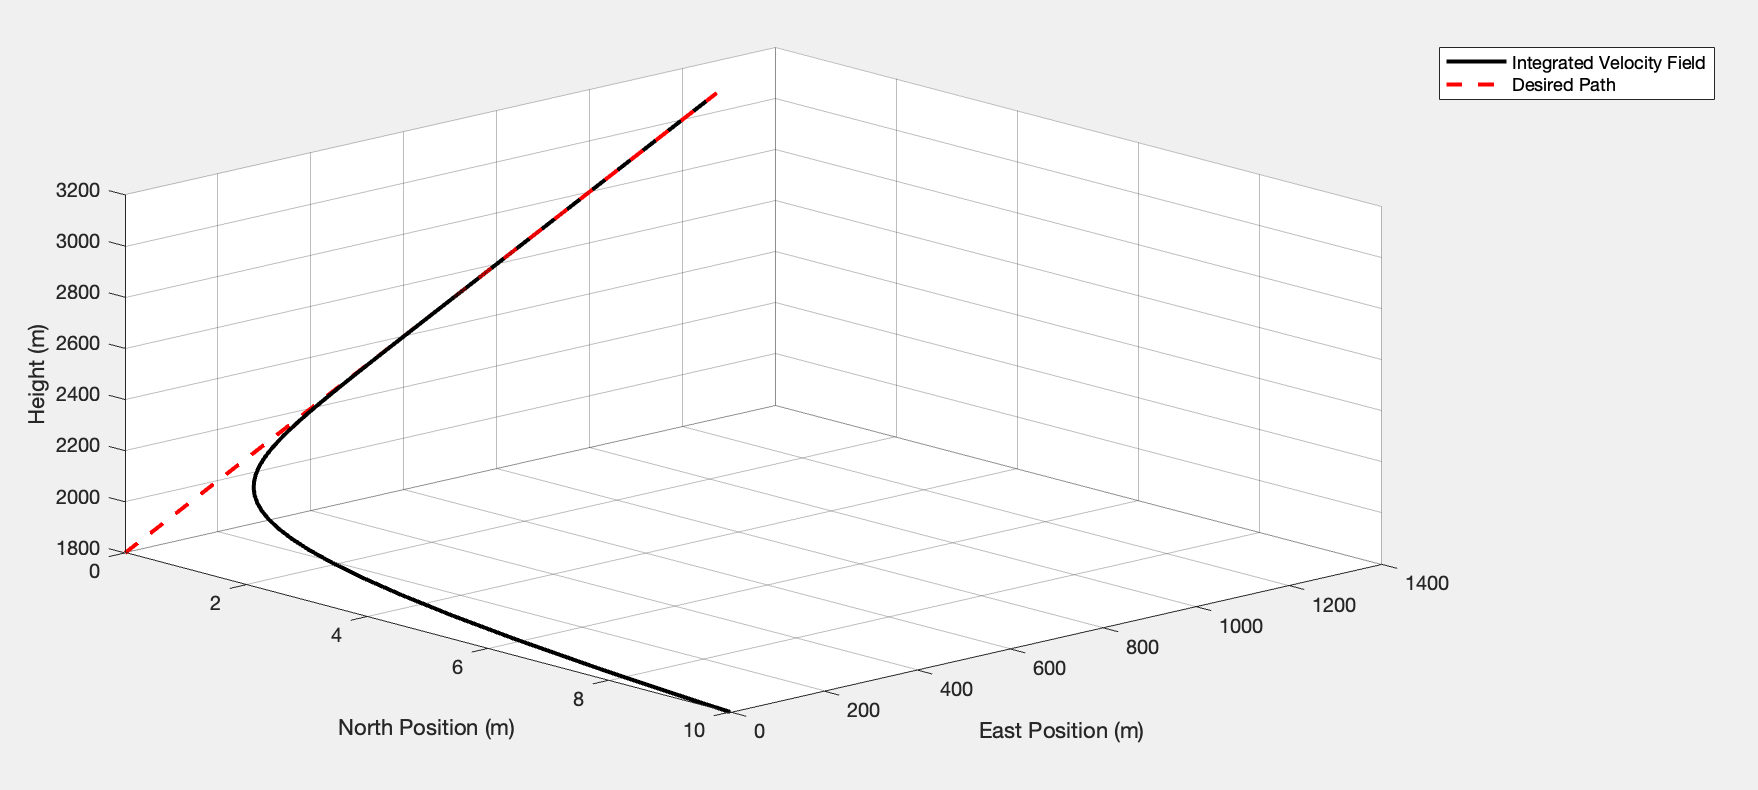
\includegraphics[width=0.5\textwidth]{images/lookahead_point.jpeg}
    \caption{Lookahead Guidance Simulation. Assuming point mass kinematics.}
    \label{fig:lookahead_sim}
\end{figure}

Thus, if the autopilot is able to correctly control based on desired heading, desired height, and desired height rate, we can command a UAS to follow a guidance line.

\subsection{UAS Autopilot Model}

The autopilot each UAS will be using is a successful loop closure controller, simulated in MATLAB.
The control block diagram for both the lateral and longitudal autopilot are shown in Figures~\ref{fig:lateral_autopilot} and~\ref{fig:longitudal_autopilot}, respectively.

\begin{figure}[h]  
    \centering
    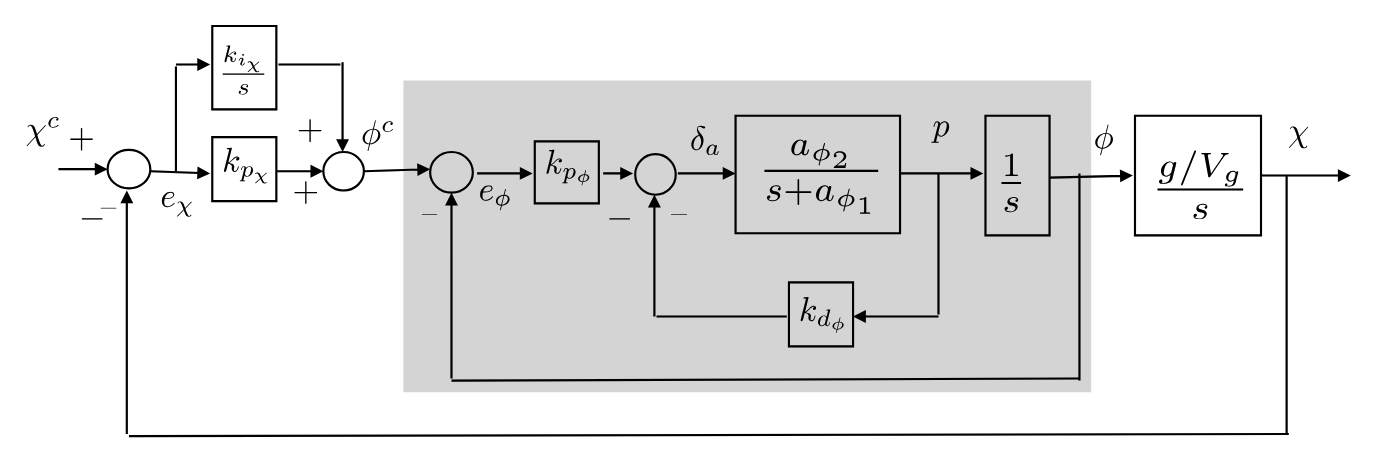
\includegraphics[width=0.5\textwidth]{images/lateral_auto.png}
    \caption{Lateral Autopilot Control Block Diagram}
    \label{fig:lateral_autopilot}
\end{figure}

\begin{figure}[h]  
    \centering
    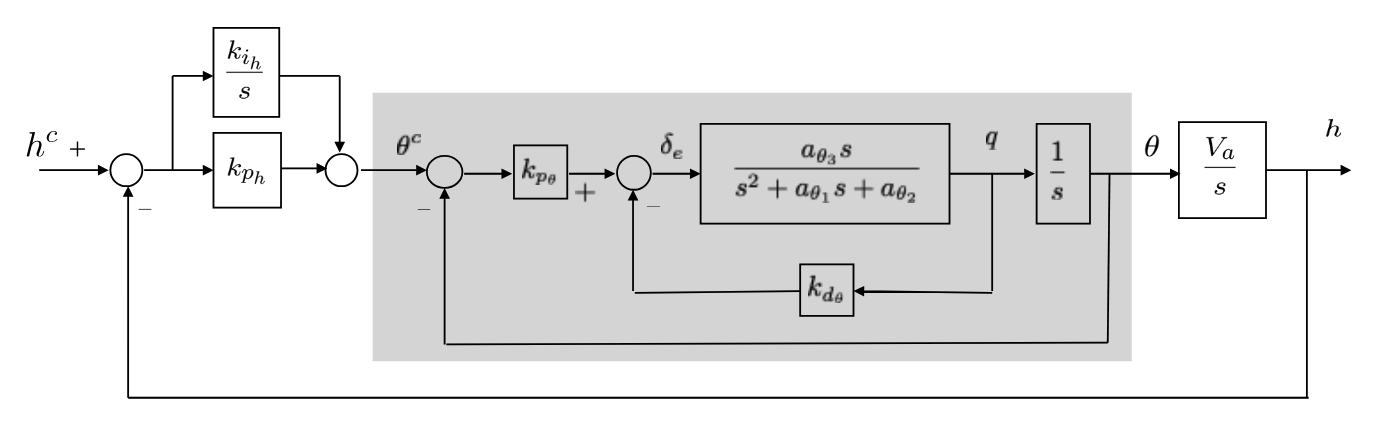
\includegraphics[width=0.5\textwidth]{images/long_auto.png}
    \caption{Longitudal Autopilot Control Block Diagram}
    \label{fig:longitudal_autopilot}
\end{figure}

In the lateral autopilot, the input is a desired heading, effecting the x and y position of the UAS.
In the longitudal autopilot, the input is a desired height, effecting the z position of the UAS.
For both of these autopilot systems, we will be using the successive loop closure (SLC) technique. 
The inner loops are shaded in gray, and by adjusting the gain values accordingly, we can assume that the inner loops react fast enough to be considered approximately perfect.
Thus, the outer loop can control heading and height, the high level commands, with the assumption the inner loop actuators and response are fast enough to be considered perfect.
The lookahead straight line following guidance algorithm given above outputs the heading and height desired at each iteration. 
This will be the guidance-autopilot loop used for all UAS in this paper.

\subsection{State and Wind Estimation}

In order to simulate using sensors to estimate the UAS's state and also the external wind, we will be using a combination of Extended Kalman Filters (EKFs) and low pass filters.
The state of a UAS is given by the vector:
\begin{equation}
    \mathbf{x} = \begin{bmatrix}
        \mathbf{x_E} \\
        \mathbf{y_E} \\
        \mathbf{z_E} \\
        \mathbf{\phi} \\
        \mathbf{\theta} \\
        \mathbf{\psi} \\
        \mathbf{u^{E}} \\
        \mathbf{v^{E}} \\
        \mathbf{w^{E}} \\
        \mathbf{p} \\
        \mathbf{q} \\
        \mathbf{r}\\
    \end{bmatrix}
\end{equation}

The tuple $\mathbf{x_E}, \mathbf{y_E}, \mathbf{z_E}$ is the position of the UAS in the inertial frame (north, east, down).
The tuple $\mathbf{\phi}, \mathbf{\theta}, \mathbf{\psi}$ is the euler angles for the attitude of the UAS (roll, pitch, yaw).
The tuple $\mathbf{u^{E}}, \mathbf{v^{E}}, \mathbf{w^{E}}$ is the inertial velocity in the UAS body frame (forward, right wing, down).
The tuple $\mathbf{p}, \mathbf{q}, \mathbf{r}$ is the angular velocity vector in the UAS body frame.

The position of the UAS is measured using a GPS sensor. The euler angles and angular rates are measured using a 3-axis rate gyroscope.

A low pass filter uses the following equation to filter measurements:
\begin{equation}
    \mathbf{y}_{new} = \alpha \mathbf{y}_{old} + (1 - \alpha) \mathbf{y}_{meas}
    \label{eq:low_pass}
\end{equation}

Where $\alpha$ maps to the equation $\alpha = e^{-a T_s}$. Where $a$ is the cutoff frequency and $T_s$ is the sample rate of the sensor.
This simple equation is able to filter and estimate noisy measurements by tuning the cutoff frequency. The noiser the measurement is, the lower the cutoff frequency should be, and vice versa.
A figure showing the effect of the cutoff frequency on the filtered measurement is shown in Figure~\ref{fig:low_pass}.

\begin{figure}[h]  
    \centering
    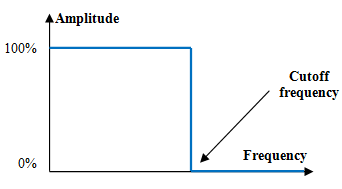
\includegraphics[width=0.4\textwidth]{images/low_pass.png}
    \caption{Low pass filter: effect of cutoff frequency on filtered measurement}
    \label{fig:low_pass}
\end{figure}

The low pass filter will be utilized to estimate the angular velocity, height, and airspeed of the UAS.
However, for the euler angles and GPS measurements, we will be using an EKF to estimate the state, as these require more complex sensor models.

The general algorithm for the EKF is given in Algorithm~\ref{alg:ekf}.

\begin{algorithm}
    \caption{Extended Kalman Filter}\label{alg:ekf}
    \begin{algorithmic}
    \State \textit{Given a system model and measurement model, predict and update the state of the system.}
    \Function{ekf}{x, P, u, z, Q, R}
    \State Predict: $\hat{x}_{k|k-1} = f(x_{k-1}, u_k)$
    \State Predict Covariance: $P_{k|k-1} = F_k P_{k-1} F_k^T + Q_k$
    \State Update: $K_k = P_{k|k-1} H_k^T (H_k P_{k|k-1} H_k^T + R_k)^{-1}$
    \State Update Estimate: $\hat{x}_k = \hat{x}_{k|k-1} + K_k (z_k - h(\hat{x}_{k|k-1}))$
    \State Update Covariance: $P_k = (I - K_k H_k) P_{k|k-1}$
    \State Return $\hat{x}_k, P_k$
    \EndFunction
    \end{algorithmic}
\end{algorithm}

The EKF works great for estimating the euler angle and GPS position measurements overtime for the UAS.
However, to estimate wind, we need to use a couple of tricks in the GPS smoothing EKF.

There is no sensor that is directly measuring the wind. But, we do have a low pass filter measuring the airspeed, $V_a$, and the GPS is able to measure the ground speed, $V_g$.
Also, we know that the way an Extended Kalman Filter works is heavily influenced by the kalman gain multiplied by the innovation. The kalman gain is the matrix $K_k$ that effectively acts as a gain for changing the estimate of the state.
The innovation is the vector $z_k - h(\hat{x}_{k|k-1})$ that represents the difference between the actual measurement, $z_k$, and the predicted measurement, $h(\hat{x}_{k|k-1})$.
Thus, the kalman gain works to drive the difference between $z_k$ and $h(\hat{x}_{k|k-1})$ to zero.

\begin{figure}[h]  
    \centering
    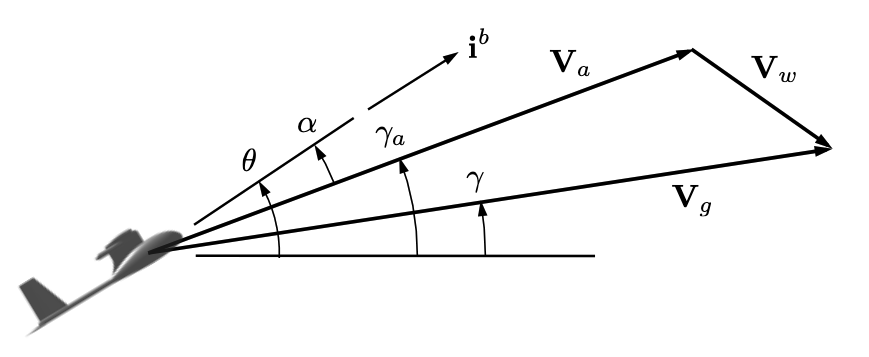
\includegraphics[width=0.4\textwidth]{images/wind_triangle.png}
    \caption{Wind triangle for a UAS, projected into the vertical plane.}
    \label{fig:wind_triangle}
\end{figure}

This concept can be exploited to estimate wind by introducting a pseudo measurement of wind.
From the wind triangle, shown in Figure~\ref{fig:wind_triangle}, we can derive the following relationships, if we assume $\gamma = \gamma_a$:

\begin{equation}
    V_a \cos(\psi) + w_n = V_g \cos(\chi)
\end{equation}
\begin{equation}
    V_a \sin(\psi) + w_e = V_g \sin(\chi)
\end{equation}

These equations can be rewritten as:
\begin{equation}
    y_{wind_n} = V_a \cos(\psi) + w_n - V_g \cos(\chi)
\end{equation}
\begin{equation}
    y_{wind_e} = V_a \sin(\psi) + w_e - V_g \sin(\chi)
\end{equation}

Therefore, we can say that we never actually estimate wind, so $z_k$ has zero value for $w_n$ and $w_e$.
But, our predicted measurement is this pseudo measurement of wind, $y_{wind_n}$ and $y_{wind_e}$.
Then, the kalman gain in the filter will choose the values of $w_n$ and $w_e$ that works to minimize the difference between $z_k$ (0s) and $h(\hat{x}_{k|k-1})$ (pseudo).
Thus, choosing the values of $w_n$ and $w_e$ that successfully completes the wind triangle with the above relationships.
This is how the EKF is able to estimate the wind in the north and east directions without every directly measuring the wind.

This results in the following state estimate for the GPS smoothing EKF:

\begin{equation}
    \hat{x}_{GPS Smoothing} = \begin{bmatrix}
        \hat{p}_{n} \\
        \hat{p}_{e} \\
        \hat{V}_{g} \\
        \hat{\chi} \\
        \hat{w}_{n} \\
        \hat{w}_{e} \\
        \hat{\psi} \\
    \end{bmatrix}
\end{equation}

While the EKF estimating the attitude measurements is simply:
\begin{equation}
    \hat{x}_{Attitude} = \begin{bmatrix}
        \hat{\phi} \\
        \hat{\theta} \\
    \end{bmatrix}
\end{equation}

From this combination of estimates from the EKF formulations along with the low pass filter estimates, the full state and wind estimate of a UAS can be filtered over time.
To see the full derivation of all matrices in the EKF, please refer to the book given in \cite{small_uas}.

\subsection{Mission Profiles and Cooperative Estimation}

% To test the impact the number of UAS has on the accuracy of the wind gradient estimation, the mission profiles tested will be a series of straight line missions.
To estimate the wind gradient for a given scenario, multiple UAS will be deployed to estimate the wind at various locations in the wind field.
Using the lookahead straight line following guidance algorithm, we will simulate multiple UAS flying in a stacked formation.
A stacked formation is a formation where the UAS are flying at straight level paths through the wind field, but at different altitudes. 
This is shown in Figure~\ref{fig:stacked_formation}.

\begin{figure}[h]  
    \centering
    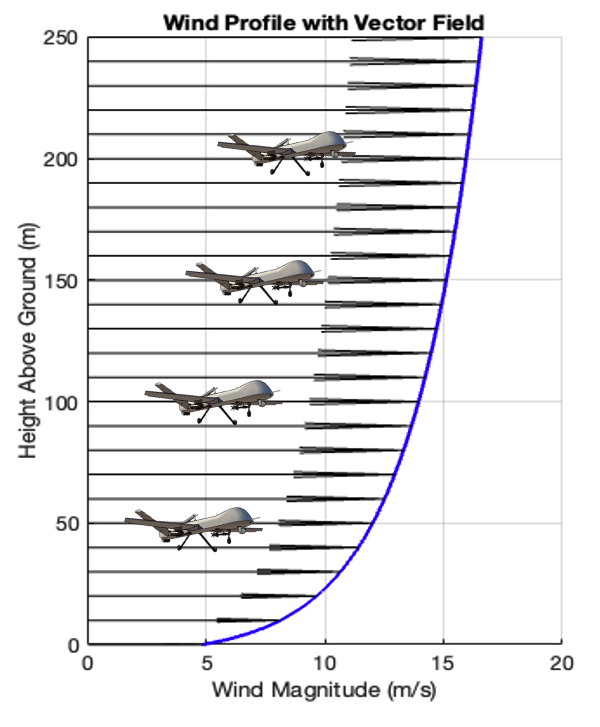
\includegraphics[width=0.4\textwidth]{images/stacked.png}
    \caption{Stacked UAS formation for estimating wind gradient.}
    \label{fig:stacked_formation}
\end{figure}



It is assumed to collabratively estimate the wind gradient, each UAS has the ability to communicate back to some centralized location; likely a ground station.
This ground station will then have online access to the state and wind estimates of all UAS at a given time step. 
Using these measurements, the wind gradient parameters $a$ and $b$ can be estimated.

\section{Solution Approach}

\subsection{Stochastic Gradient Descent}

To collabratively estimate the wind gradient, multiple UAS will share their state estimates and wind estimates to a centralized processor.
The processor will use online stochastic gradient descent to iteratively estimate the wind gradient equation given in Equation~\ref{eq:wind_gradient}.

Stochastic gradient descent (SGD) is an iterative optimization algorithm that is used to minimize a objective function of the form:

\begin{equation}
    Q(w) = \frac{1}{n} \sum_{i=1}^{n} Q_{i}(w)
\end{equation}

Where the minimizing parameter, $w$, is estimated over time.

To adapt this algorithm to the wind gradient estimation problem, we can define the following loss function:

\begin{equation}
    Loss = \frac{1}{2} (v_{i} - a log(h_{i} - b))^2
\end{equation}

Where $v_{i}$ is the estimated wind speed at the $i$th UAS and $h_{i}$ is the estimated height of the $i$th UAS.
This loss function represents the magnitude difference between the current estimated wind gradient function applied at estimated height, $a log(h_{i} - b)$, and the wind measurement that was taken, $v_{i}$.
The goal is to minimize this loss function, as this would represent a minimization of expected vs actual wind speed, much like the kalman gain being applied to the innovation term on the EKF mentioned above.

In order to do stochastic gradient descent on this loss function, we must take the derivative with respect to both parameters we need to estimate, $a$ and $b$.
The result is the following gradient equations:

\begin{equation}
    \frac{\partial Loss}{\partial a} = - (v_{i} - a log(h_{i} - b)) log(h_{i} - b)
\end{equation}

\begin{equation}
    \frac{\partial Loss}{\partial b} = - (v_{i} - a log(h_{i} - b)) \frac{a}{h_{i} - b}
\end{equation}

Now, we can descend down the gradient to minimize the loss function with the following update equations:

\begin{equation}
    a_{k+1} = a_{k} - \eta_{a} \frac{\partial Loss}{\partial a}
\end{equation}

\begin{equation}
    b_{k+1} = b_{k} - \eta_{b} \frac{\partial Loss}{\partial b}
\end{equation}

Where $\eta_{a}$ and $\eta_{b}$ are the step size or learning rates for the parameters $a$ and $b$.

Thus, the total algorithm to simulate the stacked UAS formation collaboratively estimating the wind gradient is as follows:

\begin{enumerate}
    \item Initialize a guess of $a$ and $b$
    \item Increment time step $k$
    \item For each UAS:
        \begin{enumerate}
            \item Get real wind vector from the true wind gradient given the true UAS state
            \item Using real wind and state, simulate the sensor measurements (true + noise)
            \item Use EKF and Low Pass filters to estimate the UAS state and wind vector
            \item Using estimated state and wind, get target waypoint from lookahead line guidance algorithm
            \item Input lookahead waypoint into SLC autopilot controller, outputting the control commands
            \item Using control commands, simulate the real UAS state reacting to this control, using ode45
        \end{enumerate}
    \item For each collected wind estimate, perform SGD to update the wind gradient parameters
    \item Repeat to Step 2
\end{enumerate}

This algorithm allows for online estimation of the wind gradient parameters, using iterative SGD.
All solutions shown in this paper use a $\eta_{a} = 0.01$ and $\eta_{b} = 2.5$ with an initial guess of $a = 0$ and $b = 0$.

\subsection{Estimation Parameters}

% \nsnote{here talk about the specific parameters used for low pass and ekf}
Through tuning and theory methods, the specific filter parameters we will use for this simulation are as follows:

\textbf{Low Pass Filter:}

Cutoff frequency:
\begin{itemize}
    \item $a_{\omega} = 1000$
    \item $a_{h} = 10$
    \item $a_{V_{a}} = 30$
\end{itemize}

\textbf{Extended Kalman Filter:}

\begin{equation}
    \mathbf{Q_{Attitude}} = \begin{bmatrix}
        0.01 \frac{pi}{180} ^ 2 & 0 \\
        0 & 0.01 \frac{pi}{180} ^ 2
    \end{bmatrix}
\end{equation}
\begin{equation}
    \mathbf{R_{Attitude}} = \begin{bmatrix}
        e_{\phi \theta \psi}^2 & 0 & 0 \\
        0 & e_{\phi \theta \psi}^2 & 0 \\
        0 & 0 & e_{\phi \theta \psi}^2
    \end{bmatrix}
\end{equation}

Where:
\begin{center}
$x_{Attitude} = [\phi, \theta]$ \\
$y_{Attitude} \approx [p, q, r]$ \\
$e_{x}$ terms are known error uncertainties
\end{center}


\begin{equation}
    \mathbf{Q_{GPS}} = \begin{bmatrix}
        100 & 0 & 0 & 0 & 0 & 0 & 0 \\
        0 & 100 & 0 & 0 & 0 & 0 & 0 \\
        0 & 0 & 4 & 0 & 0 & 0 & 0 \\
        0 & 0 & 0 & 5 \frac{pi}{180} ^ 2 & 0 & 0 & 0 \\
        0 & 0 & 0 & 0 & 25 & 0 & 0 \\
        0 & 0 & 0 & 0 & 0 & 25 & 0 \\
        0 & 0 & 0 & 0 & 0 & 0 & 5 \frac{pi}{180} ^ 2
    \end{bmatrix}
    \label{eq:ekf_q_gps}
\end{equation}

\begin{equation}
    \mathbf{R_{GPS}} = \begin{bmatrix}
        e_{p_{n}}^2 & 0 & 0 & 0 & 0 & 0 \\
        0 & e_{p_{e}}^2 & 0 & 0 & 0 & 0 \\
        0 & 0 & e_{V_g}^2 & 0 & 0 & 0 \\
        0 & 0 & 0 & \frac{e_{V_g}}{20}^2 & 0 & 0\\ 
        0 & 0 & 0 & 0 & e_{V_{g}}^2 & 0 \\
        0 & 0 & 0 & 0 & 0 & e_{V_{g}}^2 
    \end{bmatrix}
\end{equation}

Where:
\begin{center}
$x_{GPS} = [p_{n}, p_{e}, V_{g}, \chi, w_n, w_e, \psi]$ \\
$y_{GPS} \approx [p_{n}, p_{e}, V_{g}, \chi, w_n, w_e]$ \\
$e_{x}$ terms are known error uncertainties
\end{center}

\subsection{Adjusting the Extended Kalman Filter}

It is important to note that the EKF implementation presented in the Problem Formulation section makes the assumption that the wind measurement is constant with time.
The transition function for the wind state is set to:

\begin{equation}
    \dot{w}_n = 0
\end{equation}

\begin{equation}
    \dot{w}_e = 0
\end{equation}

This assumption is valid for steady state wind conditions, but, for this problem, we need to be careful with this assumption.
Although the wind gradient is constant, the magnitudes of wind vary with altitude. 
Thus, as the UAS drift up and down, which happens even though we are commanding a straight line path because there is sensor and autopilot noise, the wind magnitude will change.
This changing wind magnitude is especially prevalent in large wind gradients, or in UAS flying at a low altitude, as that is where the gradient is the largest, as seen in Figure~\ref{fig:wind_gradients}.

To account for this, we can adjust the EKF matrices to be less confident in the assumption that wind is steady state.
This can be done by increasing the diagonal elements of the process noise covariance matrix, $\mathbf{Q}$, for the wind predictions. 
By increasing the process noise, the assumption that wind is steady state in the transition function has less weight, and the EKF is less confident in updating the wind according to that assumption. 
This allows the EKF to work better in the presence of changing wind magnitudes as the UAS traverses the gradient. Even though we are still making the assumption that wind is steady state, we are not as confident in it.

Specially, I found that increasing the 5th and 6th diagonal elements of the Q given in Equation~\ref{eq:ekf_q_gps} to 150 instead of 25 was able to account for the changing wind magnitudes in a wind gradient.
This worked up to wind gradients with an $a$ value of 15, which is a very strong gradient. If you wish to use this EKF implementation in a stronger wind gradient, you will likely need to increase the process noise even more.

\section{Results}

\subsection{Basic Results}

The first example we will show is 3 UAS estimating a wind gradient with an $a = 1.5$ and $b = 10$.
The wind direction is assumed to be in the [1, 1, 0] inertial direction.
These UAS are initalized and commanded to follow a series of lines 25 feet apart and off the ground.
Thus, there is a UAS flying at 25 m, 50 m, and 75 m from the ground.
The aircraft will be simulated for 50 seconds, with a speed of 18 m/s and an EKF update rate of 1 Hz.
The trajectories of the aircraft can be seen in Figure~\ref{fig:uas_traj_three}.

\begin{figure}[h]
    \centering
    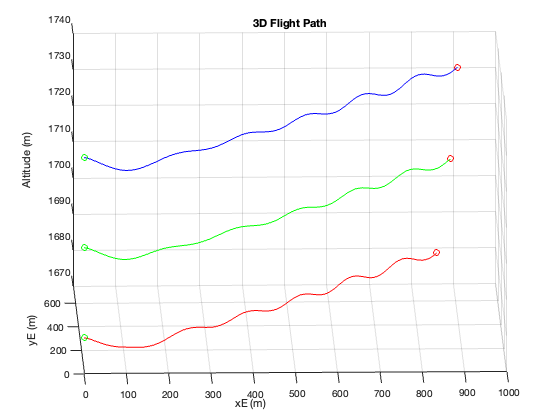
\includegraphics[width=0.5\textwidth]{images/uas_traj_3.png}
    \caption{Trajectories of 3 UAS spread apart by 25 m guidance lines. Flying in a wind gradient with $a = 1.5$ and $b = 10$ in the [1, 1, 0] inertial direction.}
    \label{fig:uas_traj_three}
\end{figure}

As you can see from the figure, the UAS are able to accurately follow their straight, level, guidance lines with only some oscillations.

Now, looking at the estimated wind gradient figures we can see the progression difference between 2.5 seconds vs 7 seconds vs 15 seconds into the simulation.
These can be seen in Figures~\ref{fig:uas_traj_three_25}, ~\ref{fig:uas_traj_three_75}, and ~\ref{fig:uas_traj_three_15}.

\begin{figure}[h]
    \centering
    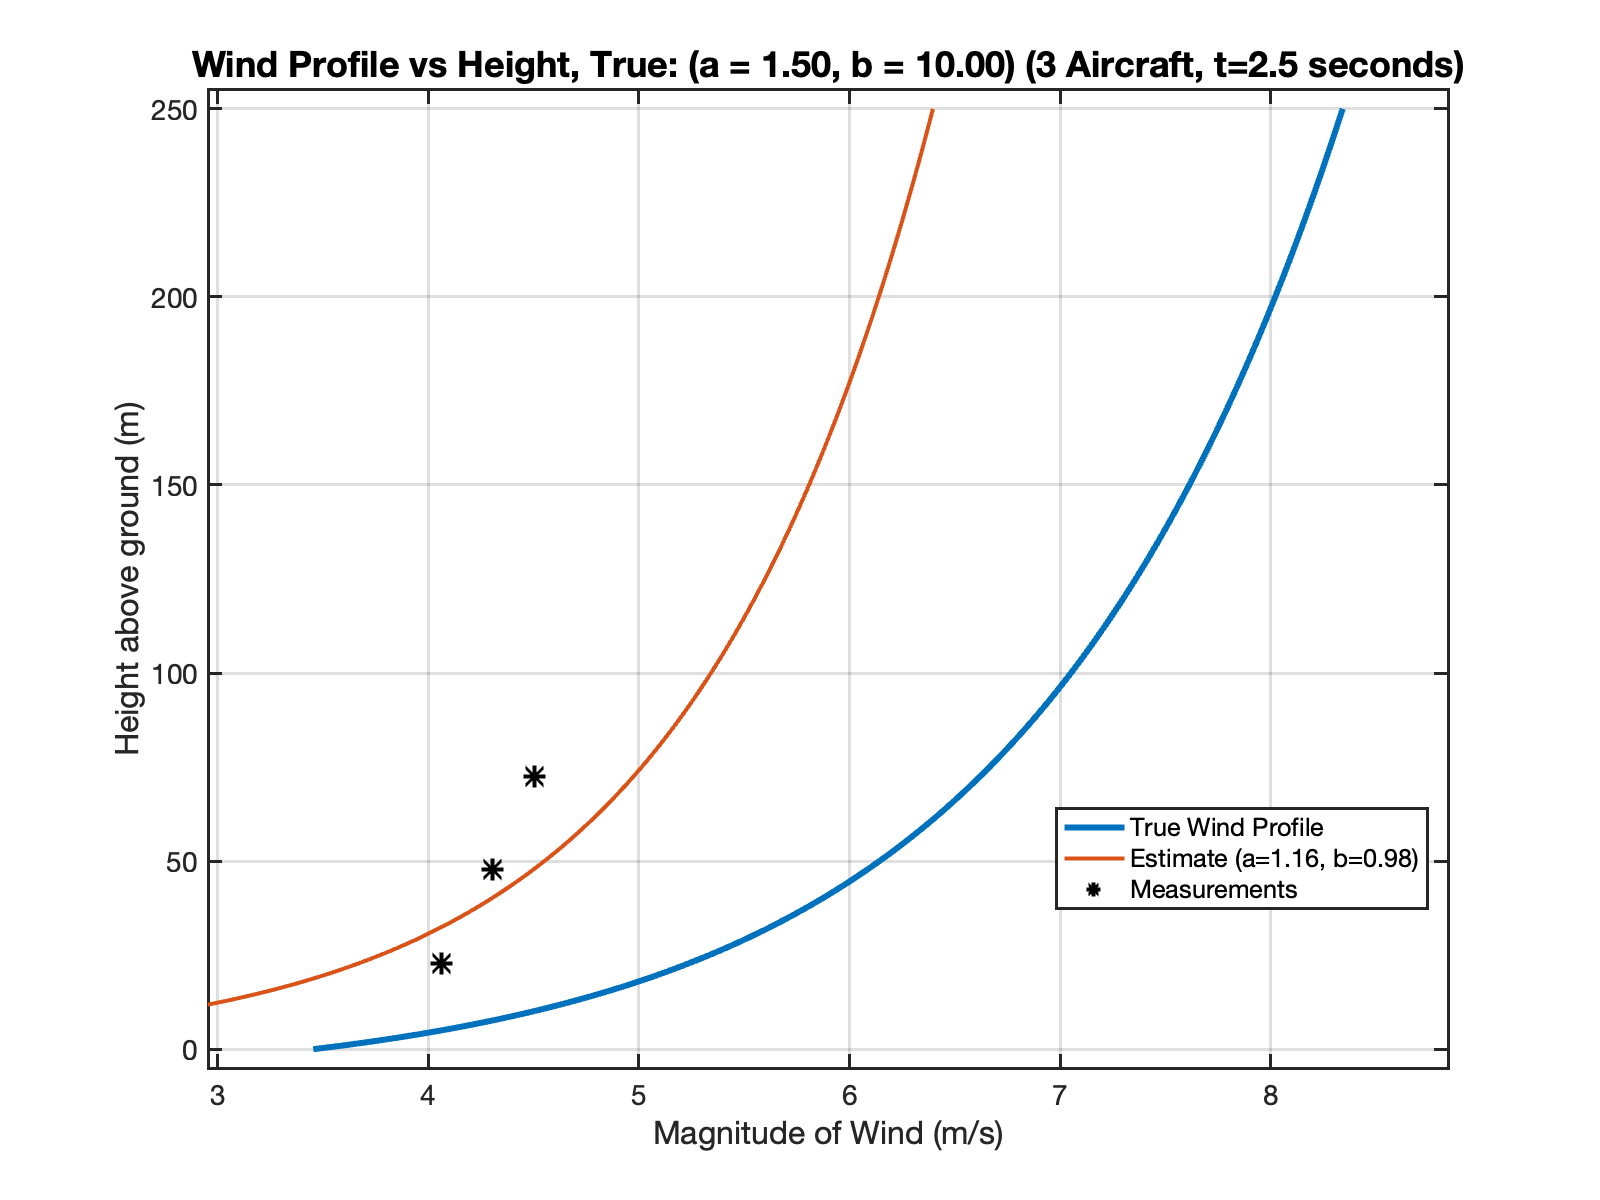
\includegraphics[width=0.5\textwidth]{images/3_uas_2.5_sec.png}
    \caption{3 UAS, estimated wind gradient after 2.5 seconds into the simulation.}
    \label{fig:uas_traj_three_25}
\end{figure}

\begin{figure}[h]
    \centering
    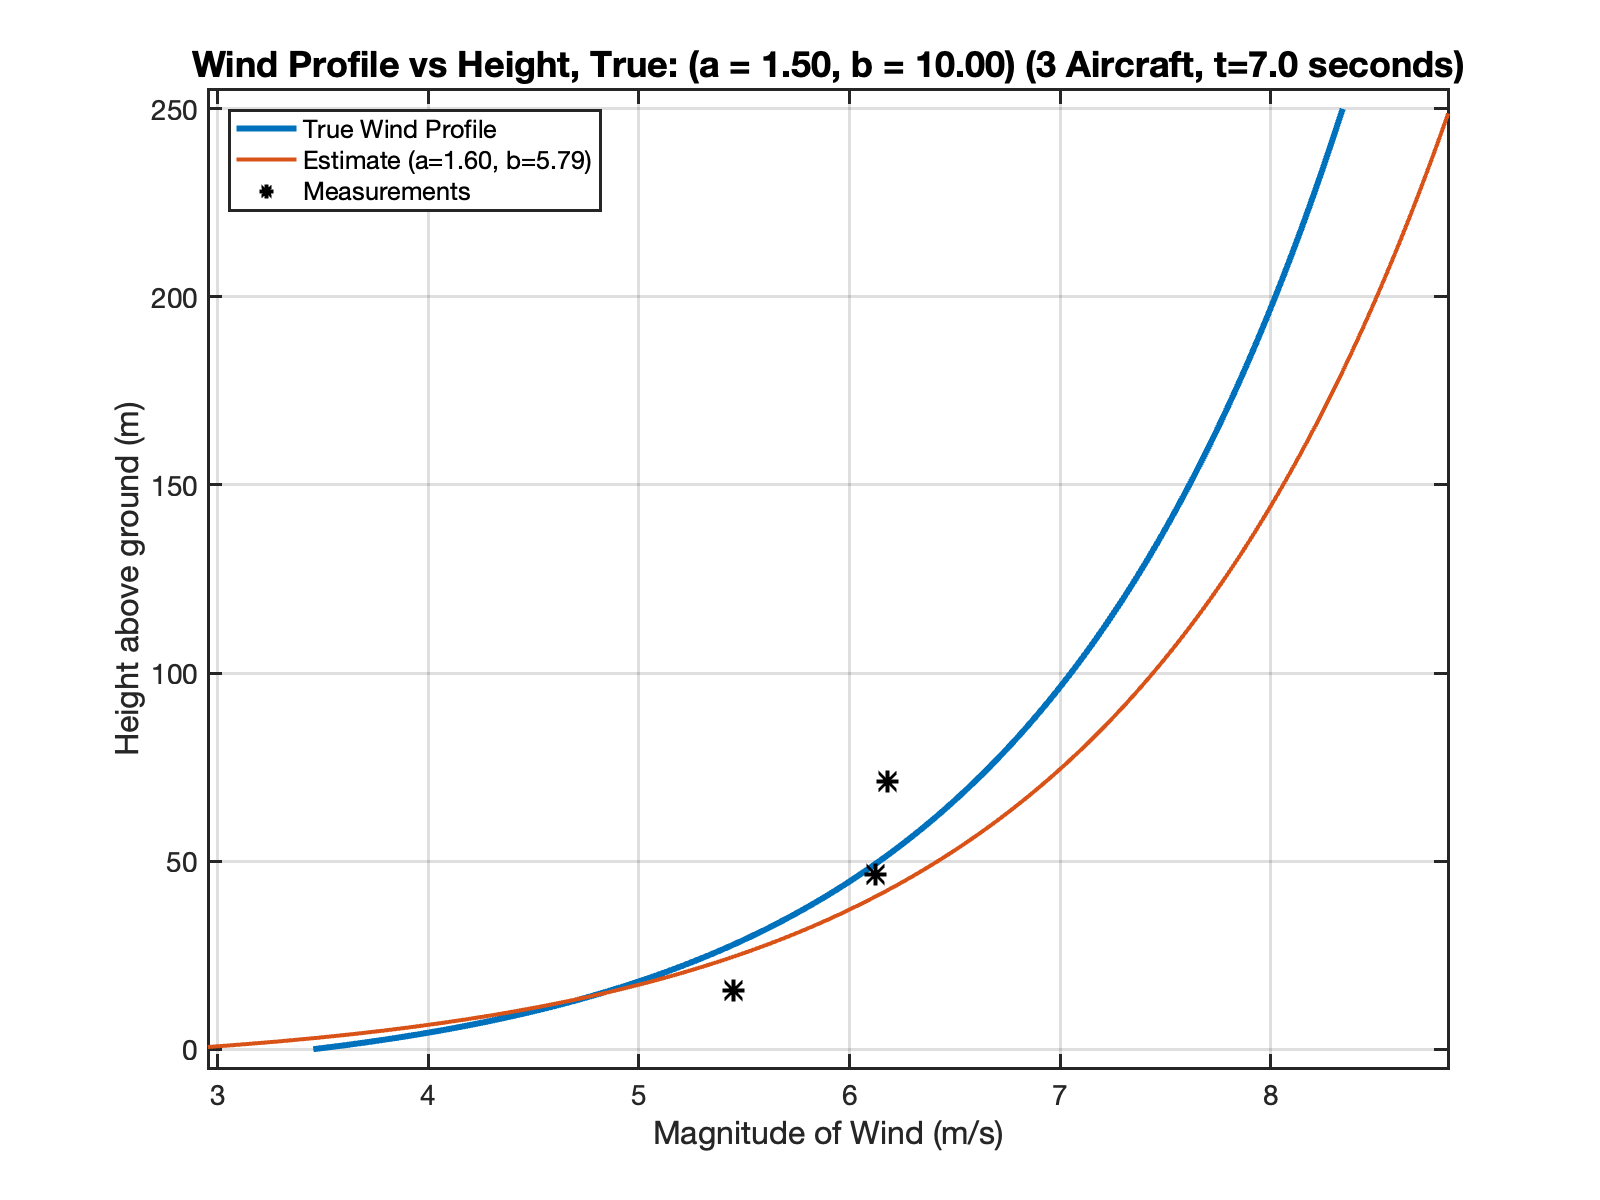
\includegraphics[width=0.5\textwidth]{images/3_uas_7_sec.png}
    \caption{3 UAS, estimated wind gradient after 7 seconds into the simulation.}
    \label{fig:uas_traj_three_75}
\end{figure}

\begin{figure}[h]
    \centering
    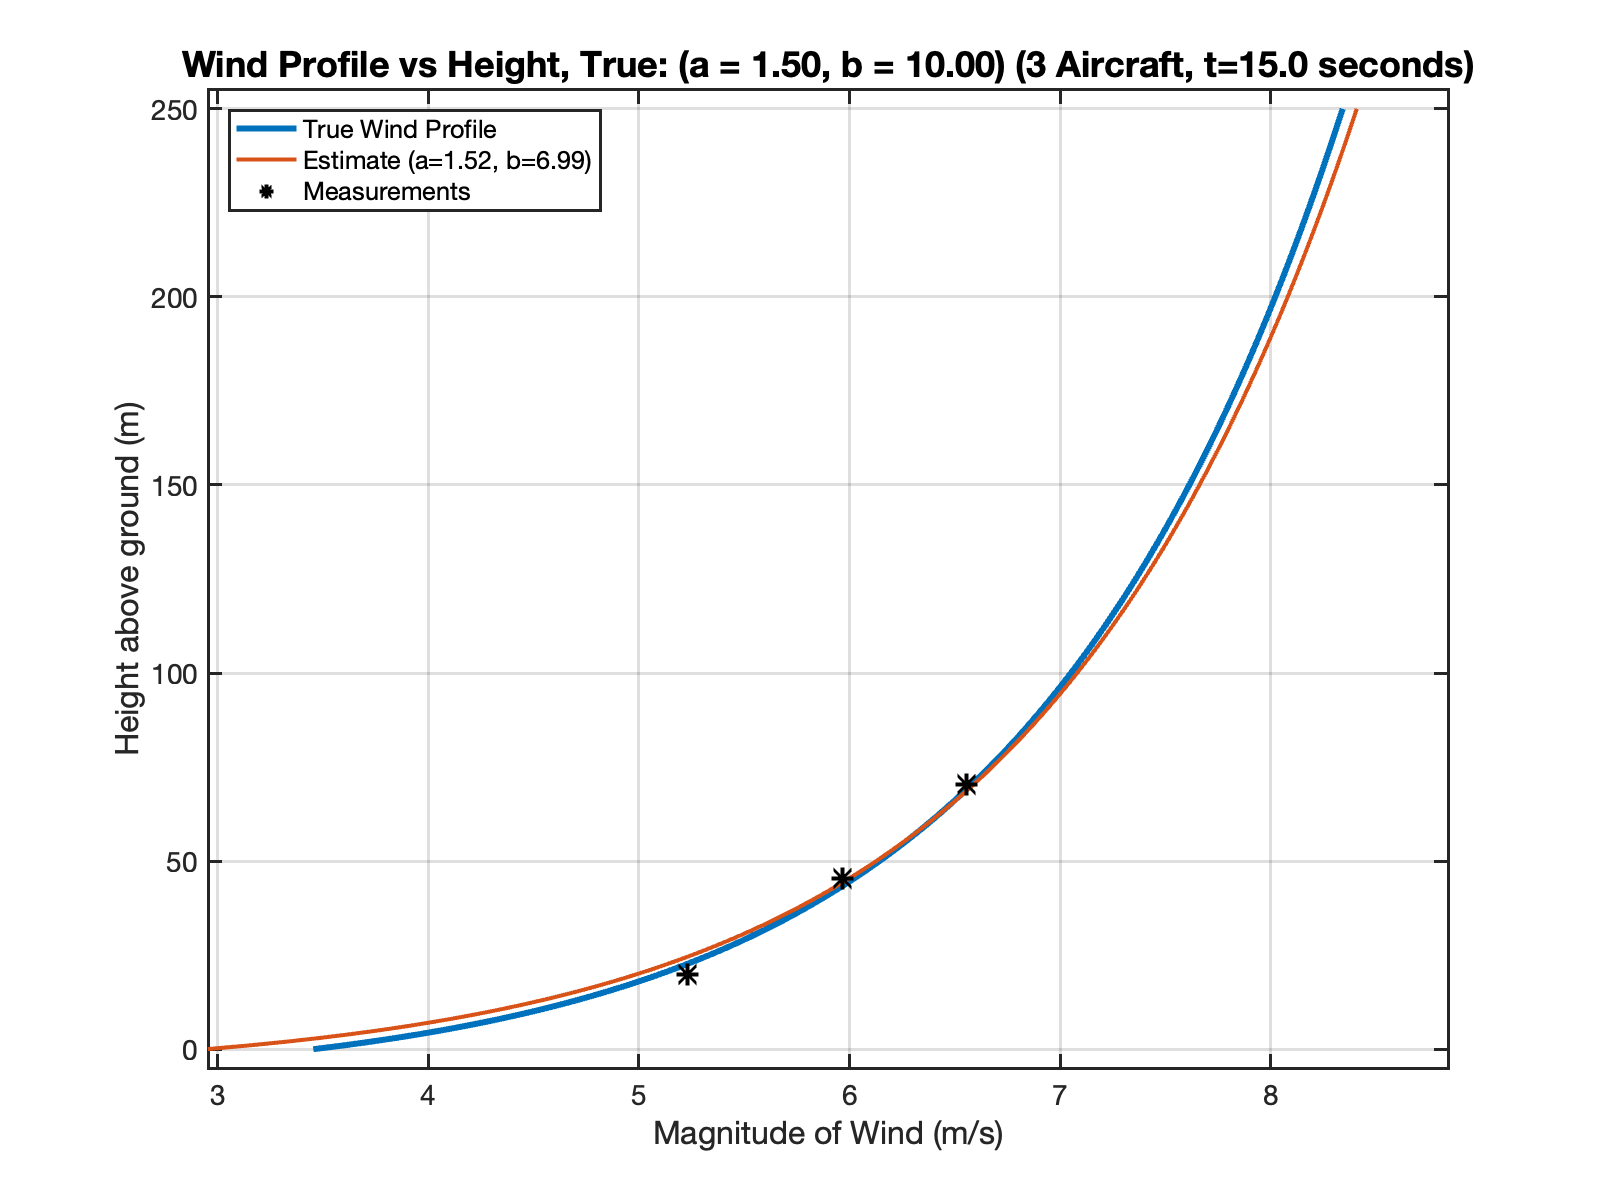
\includegraphics[width=0.5\textwidth]{images/3_uas_15_sec.png}
    \caption{3 UAS, estimated wind gradient after 15 seconds into the simulation.}
    \label{fig:uas_traj_three_15}
\end{figure}

The blue line represents the true wind gradient field that is impacting the UAS during flight.
The red line represents the current time estimate of the wind gradient field, using the $a$ and $b$ values specified in the legend.
The scatter points represent the current time estimate of a UAS position and the wind magnitude at that position.

Theres three interesting things to observe that are occuring as time progresses.
First, the UAS are able to gain steady altitude flight; correctly following their guidance lines. 
You can see in Figure~\ref{fig:uas_traj_three} that the UAS flight paths have the biggest oscillations at the start of the simulation before they steady out.
Second, as time progresses, each UAS is able to estimate its own wind field more accurately.
The difference between time 2.5 and 7 seconds shows how the scatter dots representing the UAS measured height and wind magnitude is much more accurate in the wind (x-axis) measurement.
Third, as follows from each UAS being able to accurately estimate their own wind magnitude, the overall estimated relationship of the wind gradient field begins to converge to the true wind gradient field.

This result is really a cumulative sum of all three relationships. As the UAS's autopilot is able to level out to the guidance line commanded, 
the wind measurements become more steady as the UAS is not traversing the gradient (as touched on in the \textit{Adjusting the EKF} section).
This allows the EKF to more accurately estimate the individual UAS wind measurements at that commanded height. 
With a continous stream of accurate individual wind measurements, the stochastic gradient descent algorithm can accurately converge to the correct $a$ and $b$ values that describe the true wind gradient field.
Thus, all 3 systems: the UAS autopilot, the wind EKF, and the central gradient estimator work together to accurately estimate the wind gradient field.

A video showing the full simulation over 50 seconds can be seen in the link at the top of the paper.

\subsection{Single UAS Edge Case}

An interesting edge case to consider is if this algorithm is able to successfully estimate the wind gradient with only a single UAS.
The series of results showing the same wind gradient as above, but, now with only a single UAS commanded to fly at 25 m above the ground can be seen in the Figures~\ref{fig:uas_traj_one_5} and~\ref{fig:uas_traj_one_15}.

\begin{figure}[h]
    \centering
    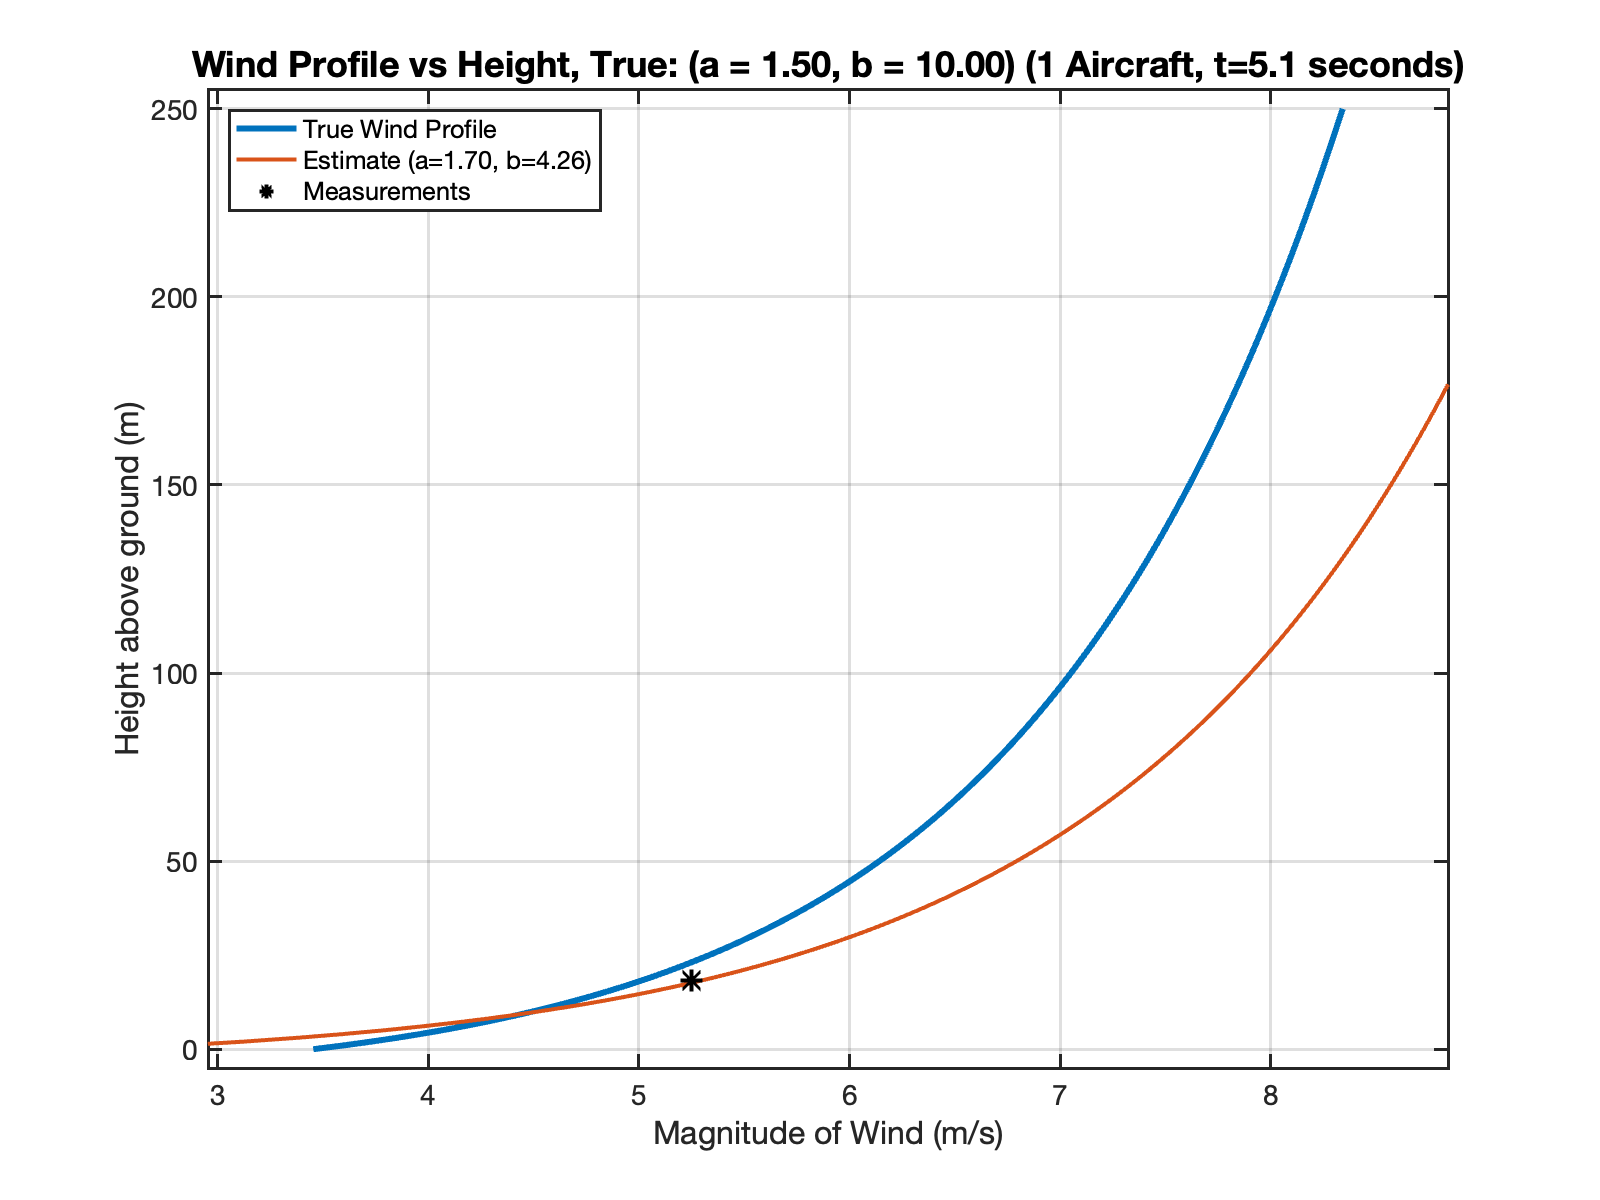
\includegraphics[width=0.5\textwidth]{images/single_5_sec.png}
    \caption{1 UAS, estimated wind gradient after 5 seconds into the simulation.}
    \label{fig:uas_traj_one_5}
\end{figure}

\begin{figure}[h]
    \centering
    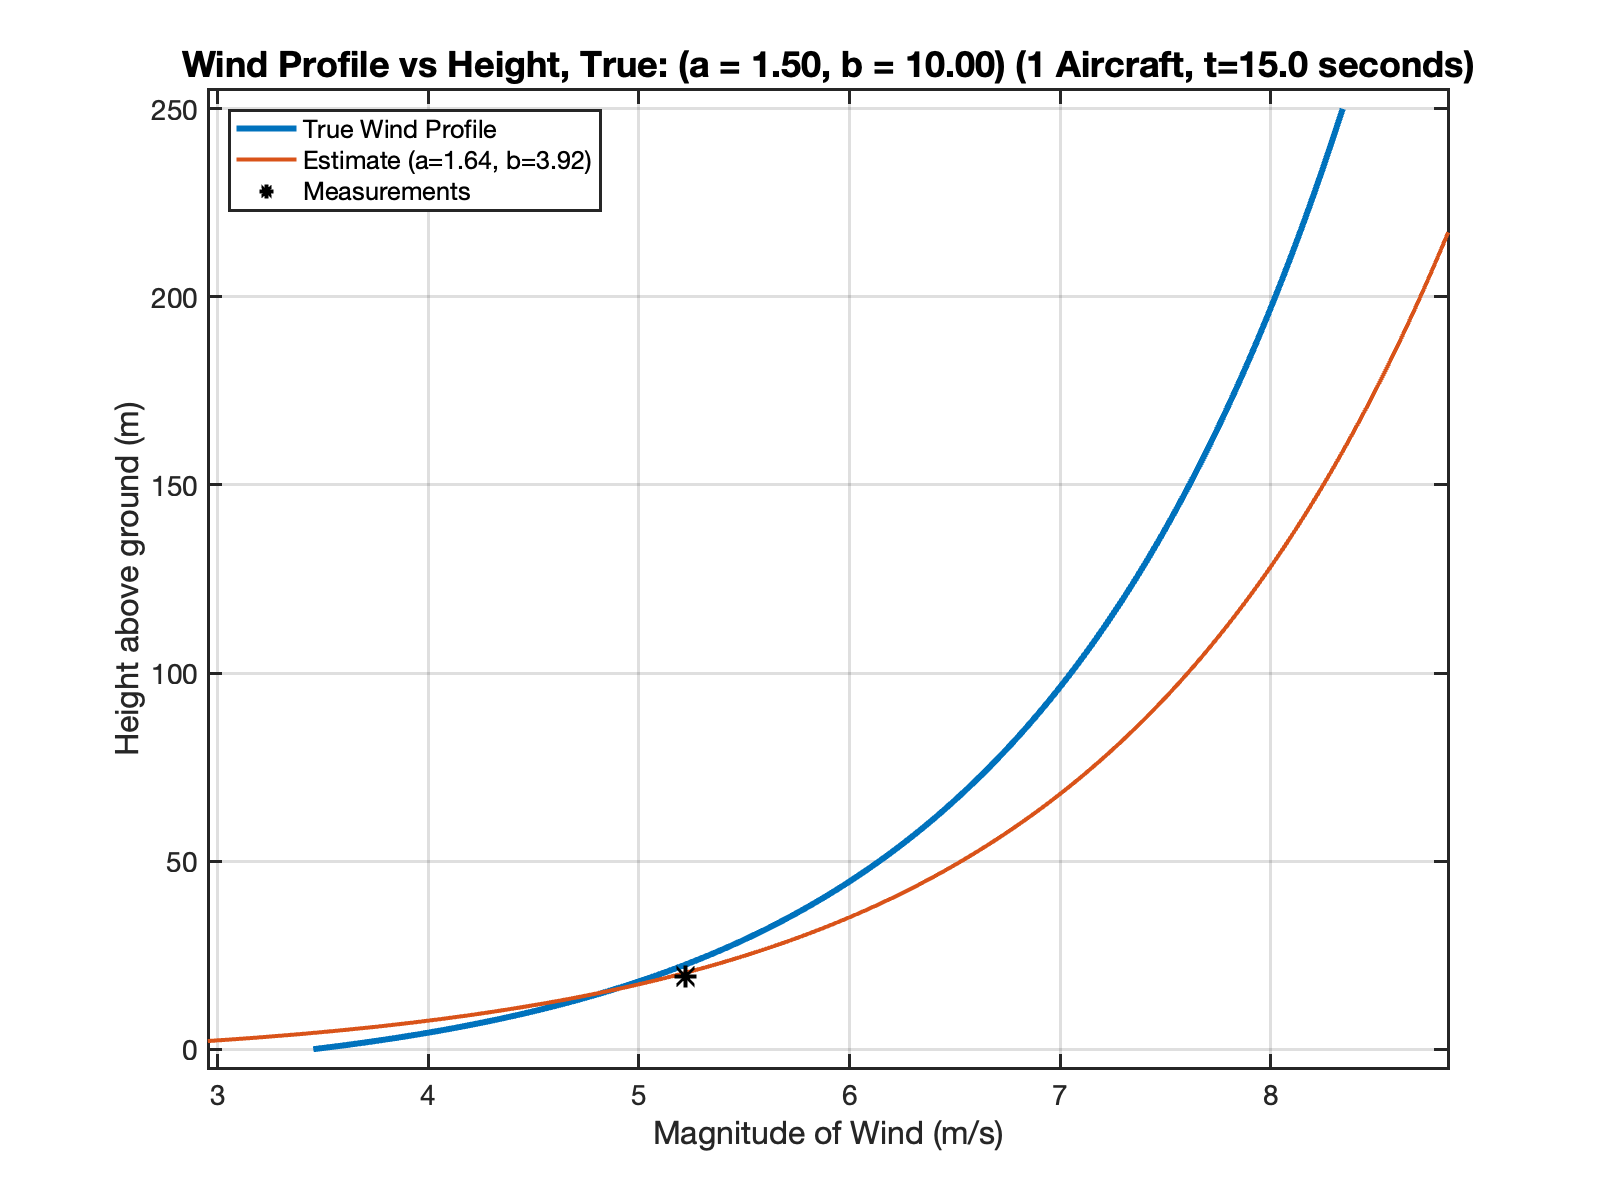
\includegraphics[width=0.5\textwidth]{images/single_15_sec.png}
    \caption{1 UAS, estimated wind gradient after 15 seconds into the simulation.}
    \label{fig:uas_traj_one_15}
\end{figure}

The results show the single UAS is able to correctly estimate its independent wind magnitude but not the entire gradient field.
By 15 seconds into the simulation, the UAS has a very accurate estimate of its own wind magnitude, as you can see the scatter point is almost exactly on the blue line showing the true wind. 
However, comparing 5 seconds vs 15 seconds, there is almost no improvement to the overall wind gradient estimation.
This is because the wind gradient the UAS has estimated is highly accurate to its singular measurement it knows.
This is the issue with only using a single UAS to estimate a wind gradient field; you only have a single observation point, which can lead to an inaccurate curve fit as there are infinite curves that could exist through that singular point.

A video showing the full simulation over 50 seconds for the single UAS case can be seen in the link at the top of the paper.

\subsection{Comparing Number of UAS}

To finalize the comparison and impact of using multiple UAS to estimate the wind gradient, we will compare the performance across a range of UAS.
Using a monte carlo simulation across 50 random wind gradient fields, with $a$ ranging from 1 to 5 and $b$ ranging from 1 to 25, we can average the difference between the true wind gradient and the estimated wind gradient for each number of UAS.
Each simulation will be ran for 50 seconds and the difference between the true and estimated gradient will be the average norm difference at the end of the simulation summed over all meter increments from 0 to 250 meters (eval the difference between true and estimated at each meter, up to 250).
Thus, 

\begin{equation}
    \text{Error} = \frac{1}{250} \sum_{h=0}^{250} \left\| \mathbf{g}_{true}(h) - \mathbf{g}_{est}(h) \right\|_2
\end{equation}

All UAS will be commanded to fly at a constant altitude guidance line in a stack formation of 25*(n) height above the ground.
Where n is the number of UAS, meaning all UAS will be spaced 25 meters apart, starting at a height of 25 meters off the ground.

The results for using 50 random wind gradient fields and averaging across all of them can be seen in Figure~\ref{fig:benchmark_num_uas}.

\begin{figure}[h]
    \centering
    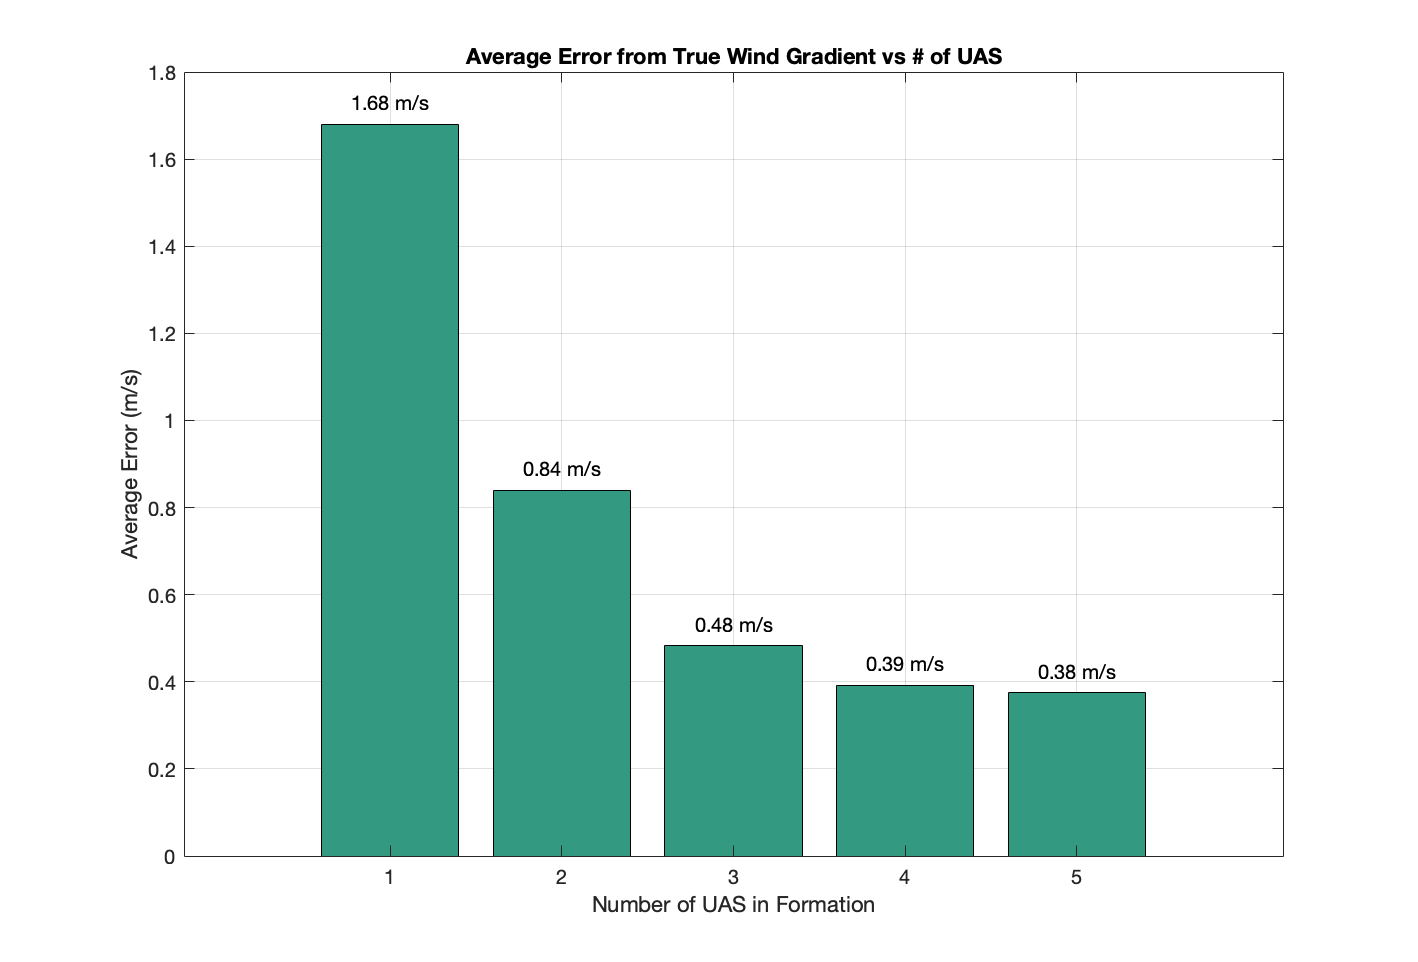
\includegraphics[width=0.5\textwidth]{images/bar_chart.png}
    \caption{Benchmarking the impact number of UAS has on estimating the wind gradient field.}
    \label{fig:benchmark_num_uas}
\end{figure}

Thus, the relationship is shown that as you increase the number of UAS flying in formation, working together to estimate the wind, the accuracy of the estimation increases.
This realtionship is quite obvious, but, its good to see the results confirm the relationship.
Its also important to see that the improvement to the estimation decreases as the number of UAS increases.
As you add more UAS, the improvement a invidiual UAS has to the overall estimation decreases. 
Therefore, depending on the application and accuracy needed in estimating the wind gradient, there is likely a sweet spot for the number of UAS to use.
Increasing the number of UAS used in a multi agent mission increases the cost and complexity of the mission and the benefits begins to decay as the number of UAS increases.


\subsection{Single UAS with a Climb Rate}

A final case we can consider is if a single UAS can accurately estimate the wind gradient if it is commanded to fly at a climb rate.
Instead of flying at a constant altitude, the UAS will be commanded to fly in a line that has a climb rate.
Specifically, we will command the UAS to follow a line specificed by the vector [1, 1, -0.5] in the inertial frame. 
Simulated over 50 seconds, the trajectory of the UAS can be seen in Figure~\ref{fig:uas_traj_one_climb}.

\begin{figure}[h]
    \centering
    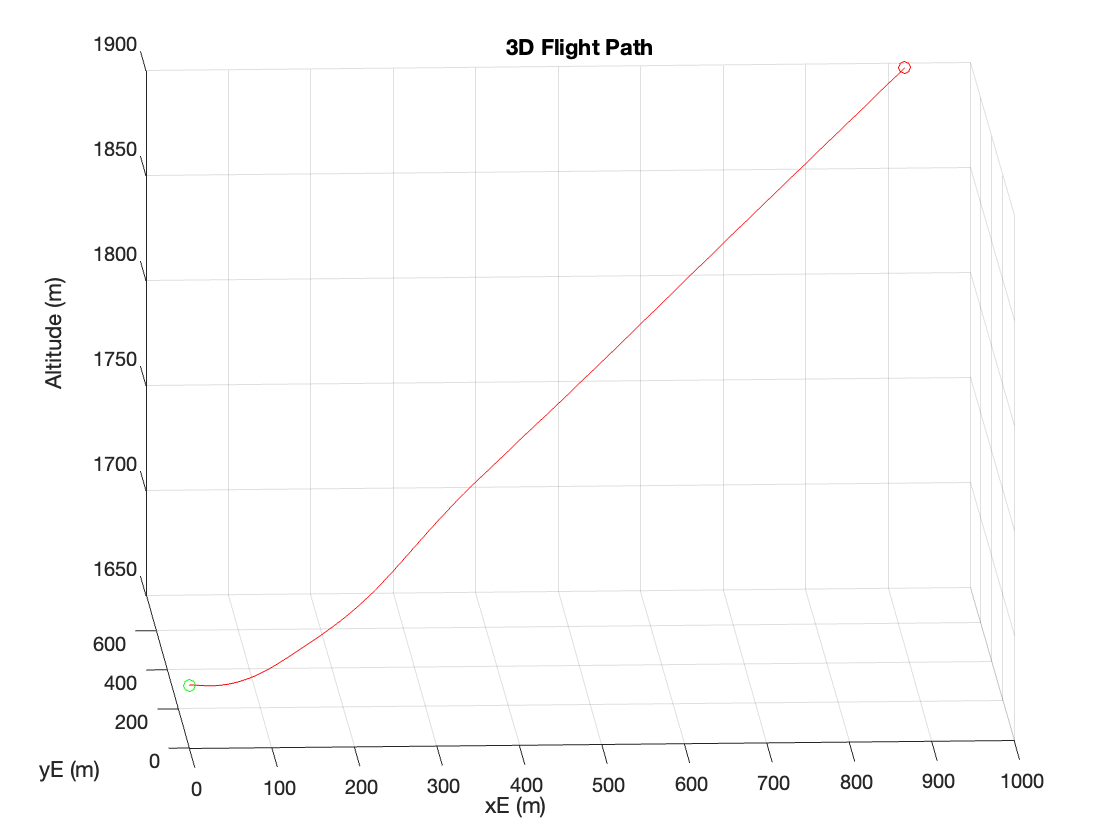
\includegraphics[width=0.5\textwidth]{images/3d_climb.png}
    \caption{3D Trajectory of a UAS following a line with a climb rate.}
    \label{fig:uas_traj_one_climb}
\end{figure}

The climb allows the UAS to traverse across the wind gradient, giving it more observability than just a single UAS flying at a constant altitude.

The results for the estimated wind gradient at 5 seconds, 20 seconds, and 40 seconds into the simulation can be seen in Figures~\ref{fig:uas_traj_one_climb_5}, ~\ref{fig:uas_traj_one_climb_20}, and ~\ref{fig:uas_traj_one_climb_40}, respectively.

\begin{figure}[h]
    \centering
    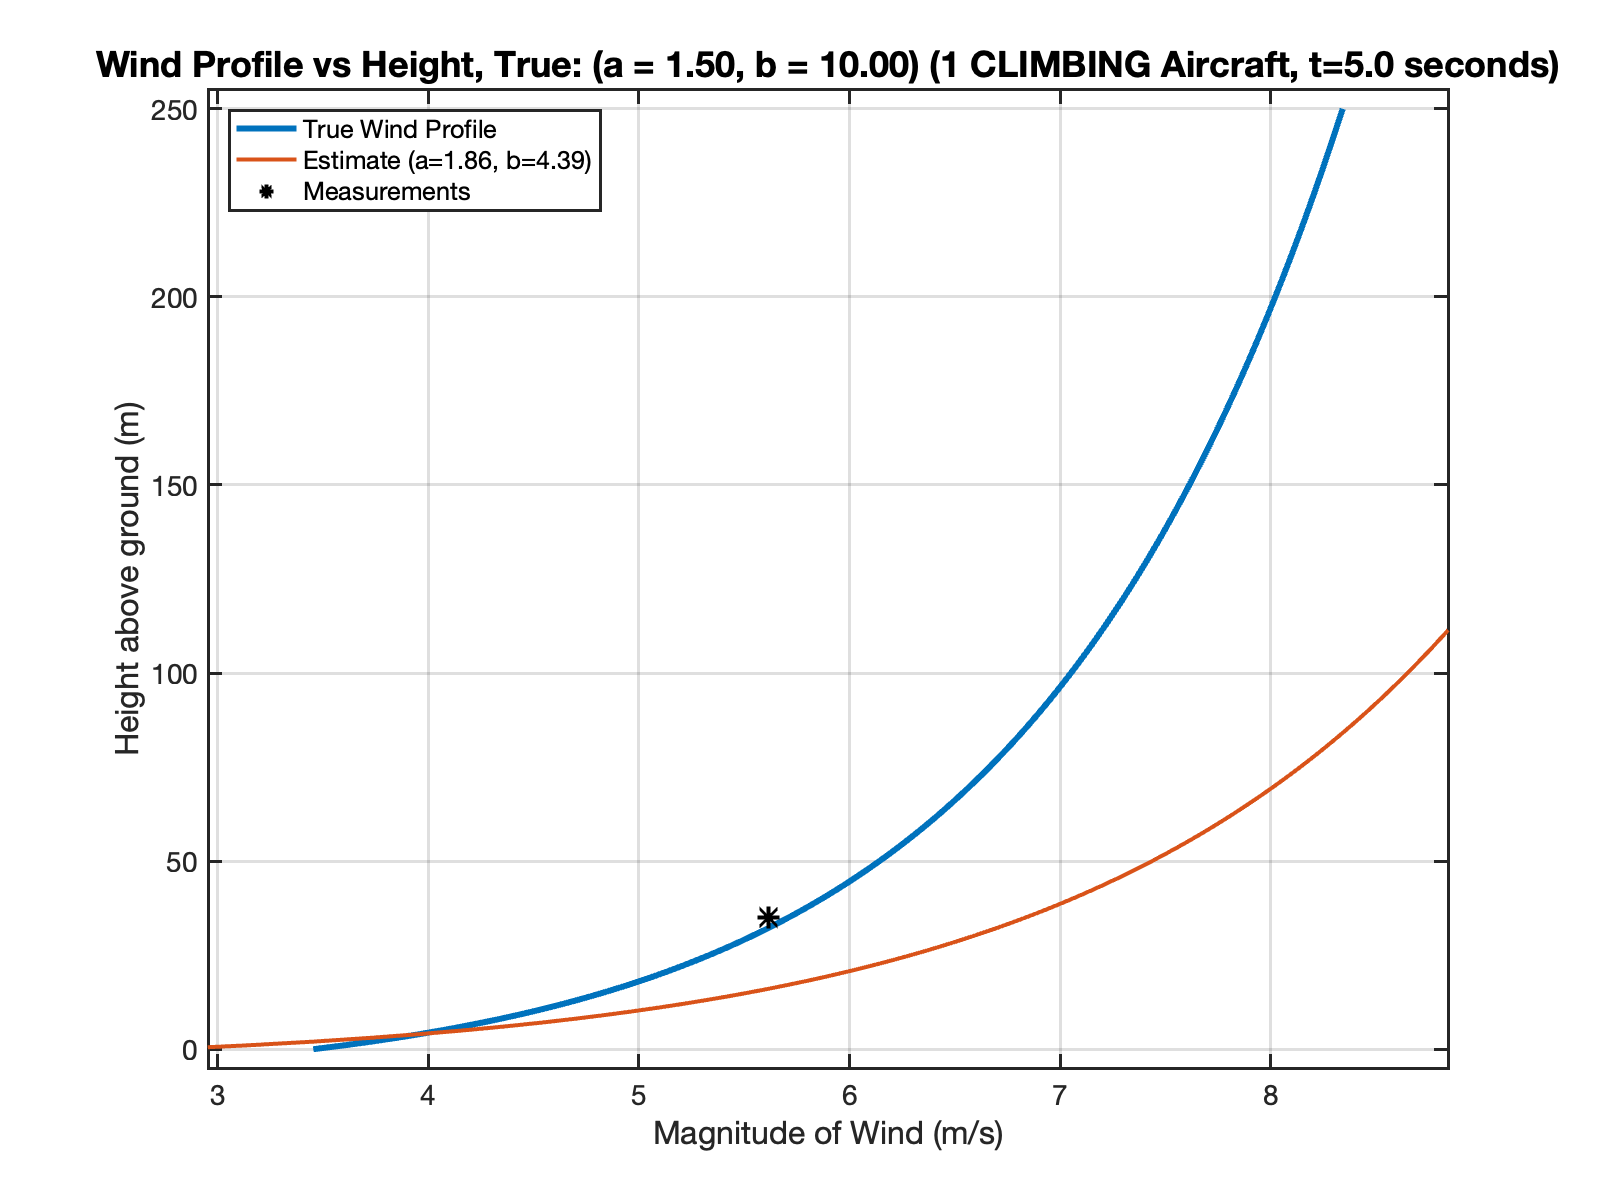
\includegraphics[width=0.5\textwidth]{images/climbing_5_sec.png}
    \caption{1 UAS, estimated wind gradient after 5 seconds into the simulation.}
    \label{fig:uas_traj_one_climb_5}
\end{figure}

\begin{figure}[h]
    \centering
    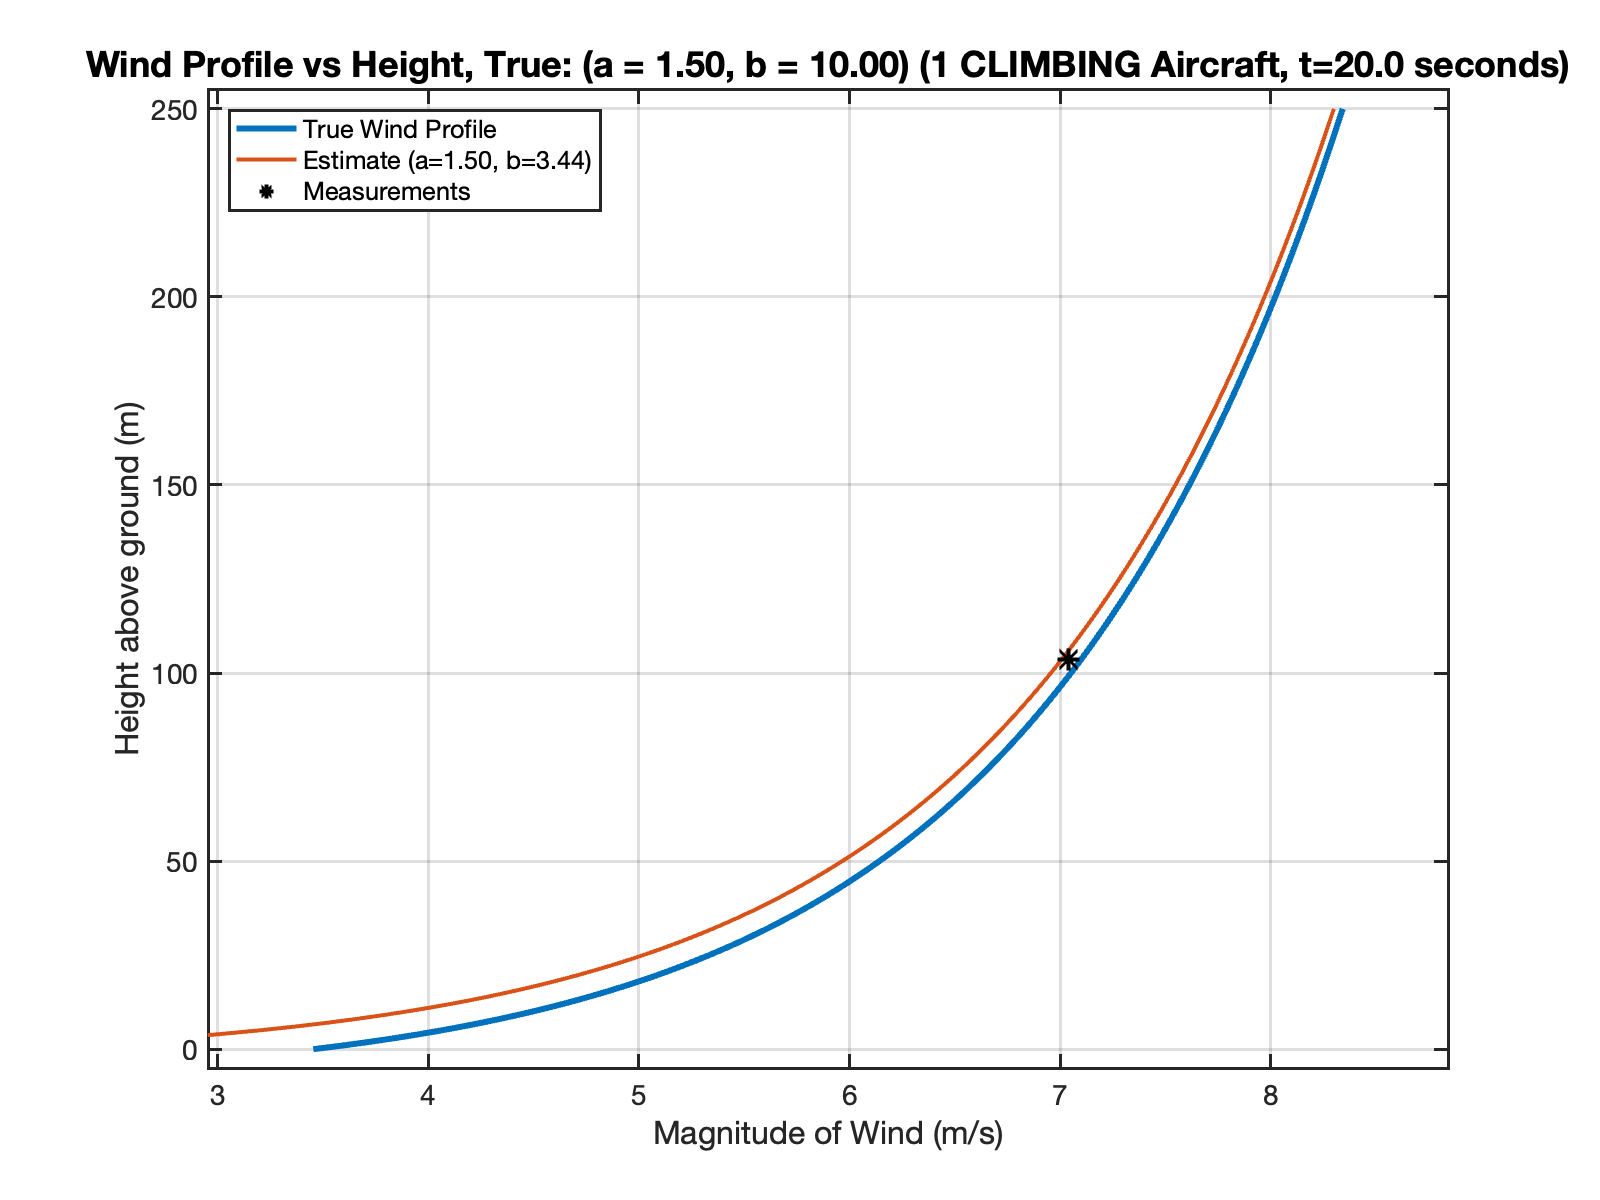
\includegraphics[width=0.5\textwidth]{images/climbing_20_sec.png}
    \caption{1 UAS, estimated wind gradient after 20 seconds into the simulation.}
    \label{fig:uas_traj_one_climb_20}
\end{figure}

\begin{figure}[h]
    \centering
    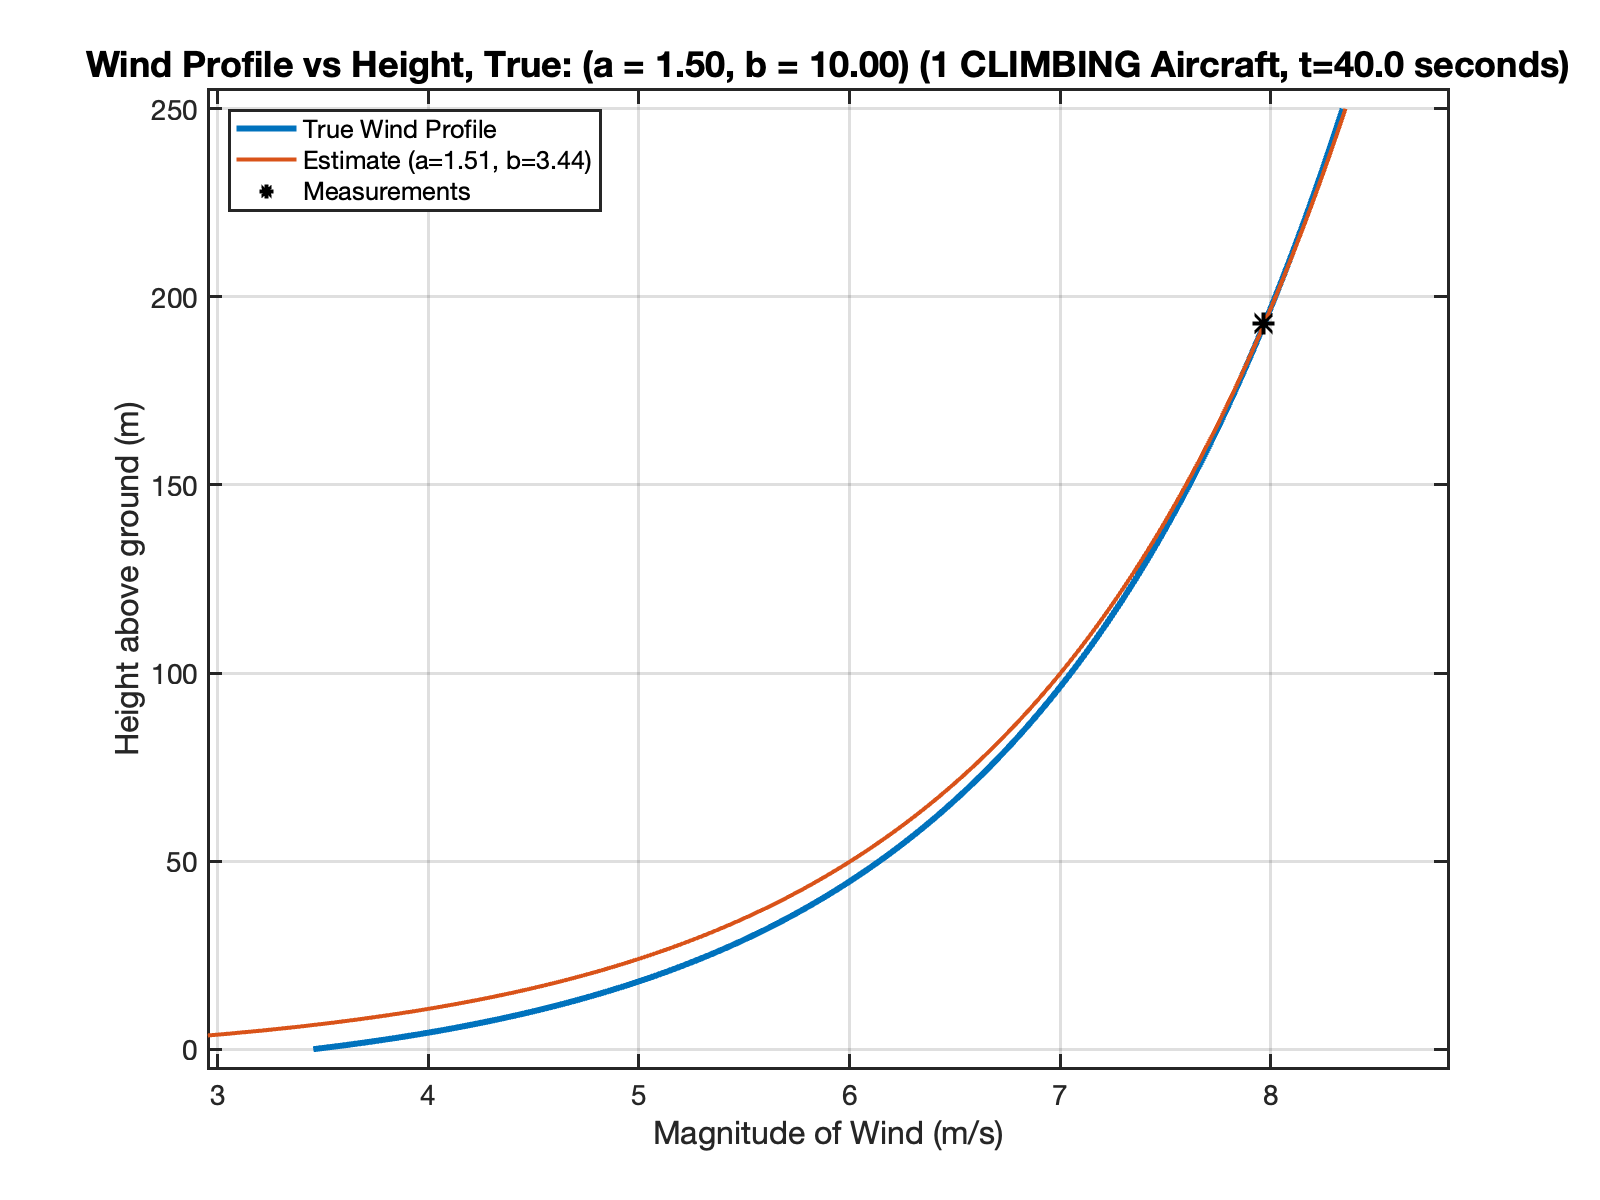
\includegraphics[width=0.5\textwidth]{images/climbing_40_sec.png}
    \caption{1 UAS, estimated wind gradient after 40 seconds into the simulation.}
    \label{fig:uas_traj_one_climb_40}
\end{figure}

As you can see from the figures, the single UAS is now able to more accurately estimate the wind gradient field, especially when compared against the constant height single UAS case seen in Figures~\ref{fig:uas_traj_one_5} and~\ref{fig:uas_traj_one_15}.
This makes sense as the issue a single UAS has is that it only has a single point of observation.
Thus, fitting a curve through that point is difficult as there are infinite solutions.
However, by commanding the UAS to climb, it is able to gain multiple observation points over time as it traverses the gradient.
This allows the online stochastic gradient descent algorithm to adjust to the entire profile of the gradient field.
The performance benefit of this is massive compared to the single, constant altitude, case shown above.
For a full video showing this scenario, see the link at the top of the paper.

One potential issue with this method of surveying the gradient field is that if the EKF is not able to accurately estimate the wind the entire algorithm, and potentially the autopilot, could fail.
The EKF for estimates wind by assuming the wind does not change over time, as discussed in the \textit{Adjusting the EKF} section.
Thus, by purposly climbing through a wind gradient, we are directly violating this assumption.
In this scenario, the EKF is still able to accurately estimate the wind at a given altitude, but, if the climb rate was higher or the gradient too big, the EKF could break and woudl not be able to estimate the wind.

Another potential issue with this scenario is that a single UAS may not be able to accurately estimate the wind gradient field if it begins changing over time.
This is a scenario we will not explore in this paper, we are always assuming a constant wind gradient, but, it is important to consider.
If the wind gradient changes over time, the single UAS, even with a climb rate, will still only have a single observation point in the time dimension.
The assumption that the single agent is able to survey the entire field over time, thus, increasing its observability, is not valid if the gradient is changing. 
The UAS may reach all altitudes in the gradient, but, the measurements may not be correlated to eachother if the gradient is changing.
However, a multi UAS formation could still accurately estimate the wind gradient as it instantanously has multiple obseveration points at any given time.



\section{Conclusion}

In this paper, we introduced a coordinated methodology for estimating wind gradient fields using multiple Uncrewed Aerial Systems (UAS). 
UAS formations can be easily created using the straight line following algorithm introducted, which commands waypoints along a given line for the UAS to follow.
The sensors onboard the UAS can be filtered using low pass filters and Extended Kalman Filters (EKF). This allows for accurate autopilot control of the estimated system.
Additionally, we introducted a pseudo wind measurement formulation in the EKF that allows for a UAS to estimate the in-plane wind by using just a GPS and IMU sensor.

Once multiple UAS are flying in a formation with filtered wind measurements, a centralized online optimizer is used to estimate the wind gradient parameters.
Using stochastic gradient descent, the optimizer is able to take observations from various UAS in the wind field and estimate the wind gradient parameters.
Once the parameters are optimized, the entire profile of the wind gradient is able to be estimated. This process is quick and effective for multiple UAS, allowing for accurate wind field estimation within minutes of flying.
Not only is wind gradient estimation important for science and engineering applicaitons, but, it woud allow the UAS who are estimating the wind to utilize the gradient to extract energy from the wind, increasing flight efficiency.
The quickness of the application presented in this paper would allow for a formation of UAS to estimate the gradient fast enough online to utilize that wind energy.

Future progress could be made by incorperating estimating wind direction into the optimizer. 
This paper only included estimating the magnitude of wind vs altitude as this is the primary factor in science and engineering applications.
But, for more advanced applications, especially dynamic soaring, wind direction is just as important.
Additionally, the effectiveness of the method proposed in this paper should be investigated in a dynamic wind gradient scenario. 
This paper only included a static wind gradient, where the parameters are constant over time.
However, this is often not the case as winds gust and change direction over the course of a mission.
How the optimizer and EKFs response to this dynamic environment would be interesting to explore.


% By integrating the UAS autopilot systems with Extended Kalman Filters (EKF) and leveraging a central stochastic gradient descent algorithm, our approach effectively enhances the accuracy of wind gradient estimations. 
% The simulation results demonstrated that our system not only maintains steady wind measurements but also converges reliably to the true wind gradient parameters under various operational scenarios. 
% This collaborative framework underscores the potential of multi-agent systems in environmental monitoring and data fusion applications. 

% Future work will focus on deploying this system in real-world environments to validate its performance beyond simulations. 
% Additionally, we aim to explore the scalability of our approach by incorporating more UAS units and investigating the impact of communication constraints on the estimation accuracy. 
% Enhancing the robustness of the EKF in dynamic conditions and integrating adaptive learning mechanisms are also planned to further improve the reliability and efficiency of wind gradient estimations.

\begin{thebibliography}{00}

\bibitem{abdalla2023} A. Abdalla, W. El-Osta, Y. Nassar, W. Husien, E. Dekam, and G. Miskeen, "Estimation of Dynamic Wind Shear Coefficient to Characterize Best Fit of Wind Speed Profiles under Different Conditions of Atmospheric Stability and Terrains for the Assessment of Height-Dependent Wind Energy in Libya," Applied Solar Energy, vol. 59, pp. 343-359, Oct. 2023.

\bibitem{matiko2013} J. W. Matiko, N. J. Grabham, S. P. Beeby, and M. J. Tudor, "Review of the Application of Energy Harvesting in Buildings," Measurement Science and Technology, vol. 25, no. 1, pp. 012002, Nov. 2013.

\bibitem{rehman2008} S. Rehman and N. M. Al-Abbadi, "Wind Shear Coefficient, Turbulence Intensity and Wind Power Potential Assessment for Dhulom, Saudi Arabia," Renewable Energy, vol. 33, no. 12, pp. 2653-2660, Dec. 2008.

\bibitem{vasel2017} A. Vasel-Be-Hagh and C. L. Archer, "Wind Farm Hub Height Optimization," Applied Energy, vol. 195, pp. 905-921, Jun. 2017.

\bibitem{probst2010} O. Probst and D. Cárdenas, "State of the Art and Trends in Wind Resource Assessment," Energies, vol. 3, no. 6, pp. 1087-1106, Jun. 2010.

\bibitem{recoskie2017} S. Recoskie, E. Lanteigne, and W. Gueaieb, "A High-Fidelity Energy Efficient Path Planner for Unmanned Airships," Robotics, vol. 6, no. 4, pp. 28, Dec. 2017.

\bibitem{small_uas}“Small Unmanned Aircraft | Princeton University Press,” February 26, 2012. https://press.princeton.edu/books/hardcover/9780691149219/small-unmanned-aircraft.


\end{thebibliography}

\end{document}